%  LaTeX support: latex@mdpi.com 
%  For support, please attach all files needed for compiling as well as the log file, and specify your operating system, LaTeX version, and LaTeX editor.

%=================================================================
\documentclass[gels,article,accept,pdftex,moreauthors]{Definitions/mdpi} 
\usepackage[labelformat=simple]{subfig}
\renewcommand\thesubfigure{\normalfont(\textbf{\alph{subfigure}})}

\usepackage[textsize=small]{todonotes}
\newcommand{\ie}{{i.e.,} }
\newcommand{\cref}{c^{\ominus}}
%\newcommand{\cs}{c_{s}}
\newcommand{\kT}{k_\mathrm{B}T}
\newcommand{\kB}{k_\mathrm{B}}
\newcommand{\lb}{l_\mathrm{B}}
%\newcommand{\NA}{N_{\mathrm{A^-}}}
\newcommand{\NA}{N_{\mathrm{A}}}
\newcommand{\muna}{\mu_\mathrm{Na^+}}

\newcommand{\mucl}{\mu_\mathrm{Cl^-}}
\newcommand{\muca}{\mu_\mathrm{Ca^{2+}}}
\newcommand{\muh}{\mu_\mathrm{H^+}}
\newcommand{\mua}{\mu_\mathrm{A^-}}
\newcommand{\muha}{\mu_\mathrm{HA}}
\newcommand{\muoh}{\mu_\mathrm{OH}}

\newcommand{\cna}{c_\mathrm{Na^+}}
\newcommand{\ccl}{c_\mathrm{Cl^-}}
\newcommand{\cca}{c_\mathrm{Ca^{2+}}}
\newcommand{\ch}{c_\mathrm{H^+}}
\newcommand{\cp}{c_\mathrm{p}}
\newcommand{\nna}{n_\mathrm{Na^+}}
\newcommand{\ncl}{n_\mathrm{Cl^-}}
\newcommand{\Nna}{N_\mathrm{Na^+}}
\newcommand{\Ncl}{N_\mathrm{Cl^-}}

\newcommand{\ncleq}{\widetilde{N}_\mathrm{Cl^-}}
\newcommand{\nca}{N_\mathrm{Ca^{2+}}}

\newcommand{\superin}{^\mathrm{in}}
\newcommand{\subin}{_\mathrm{in}}
\newcommand{\subi}{_\mathrm{i}}

\newcommand{\gel}{^\mathrm{gel}}
\newcommand{\tot}{^\mathrm{tot}}
\newcommand{\out}{^{\mathrm{out}}}
\newcommand{\coh}{c_\mathrm{OH}}
\newcommand{\bulk}{^{\mathrm{b}}}
\renewcommand{\H}{\mathrm{H^+}}
\newcommand{\A}{\mathrm{A^-}}
\newcommand{\AH}{\mathrm{AH}}
%%%%%%%%%%%%%%%%%%%%%%%%%%%%%% LyX specific LaTeX commands.

\newcommand{\cl}{\mathrm{Cl^-}}
\newcommand{\br}{\mathrm{Br^-}}
\newcommand{\na}{\mathrm{Na^+}}
\newcommand{\h}{\mathrm{H^+}}
\newcommand{\ka}{\mathrm{K^+}}
\newcommand{\oh}{\mathrm{OH^-}}
\newcommand{\ca}{\mathrm{Ca^{2+}}}
\newcommand{\mg}{\mathrm{Mg^{2+}}}

\newcommand{\Ka}{K_{\mathrm{A}}}
\newcommand{\pKa}{\mathrm{p}\Ka}
\newcommand{\pK}{\mathrm{p}K}
\newcommand{\pH}{\mathrm{pH}}
\newcommand{\mol}{\mathrm{mol}}
\newcommand{\molperl}{\mathrm{mol/L}}
\newcommand{\kg}{\mathrm{kg}}
\newcommand{\res}{^{\mathrm{res}}}
\newcommand{\pHres}{\pH\res}
\newcommand{\pHgel}{\pH\gel}
\newcommand{\cs}{c_{\mathrm{s}}}
%\newcommand{\cs}{c_{\mathrm{salt}}}
\newcommand{\csres}{\cs\res}
%\newcommand{\Vgel}{V\gel}
\newcommand{\Vgel}{V_\mathrm{gel}}
\newcommand{\vgel}{v_\mathrm{gel}}
\newcommand{\Egel}{E_\mathrm{gel}}
\newcommand{\Sgel}{S_\mathrm{gel}}
%\newcommand{\Vgel}{V}
\newcommand{\Ngel}{N_\mathrm{gel}}
%\newcommand{\Vgeleq}{\widetilde{V}_\mathrm{gel}}}
%\newcommand{\Pgel}{P_\mathrm{gel}}
\newcommand{\Pgel}{\Pi}
\newcommand{\Pres}{P_\mathrm{res}}
\newcommand{\Pout}{P_\mathrm{out}}
\newcommand{\Vout}{V_\mathrm{out}}
\newcommand{\Eout}{E_\mathrm{out}}
\newcommand{\Sout}{S_\mathrm{out}}
%\newcommand{\Vbox}{V_\mathrm{box}}
\newcommand{\Vbox}{V_0}
\newcommand{\PE}{polyelectrolyte{}}

\newcommand{\reffig}[1]{Figure~\ref{#1}}
\newcommand{\refeq}[1]{Equation~(\ref{#1}){}}
\newcommand{\etal}{{et al.}{}}

% For posting an early version of this manuscript as a preprint, you may use "preprints" as the journal and change "submit" to "accept". The document class line would be, e.g., \documentclass[preprints,article,accept,moreauthors,pdftex]{mdpi}. This is especially recommended for submission to arXiv, where line numbers should be removed before posting. For preprints.org, the editorial staff will make this change immediately prior to posting.

%--------------------
% Class Options:
%--------------------
%----------
% journal
%----------
% Choose between the following MDPI journals:
% acoustics, actuators, addictions, admsci, adolescents, aerospace, agriculture, agriengineering, agronomy, ai, algorithms, allergies, alloys, analytica, animals, antibiotics, antibodies, antioxidants, applbiosci, appliedchem, appliedmath, applmech, applmicrobiol, applnano, applsci, aquacj, architecture, arts, asc, asi, astronomy, atmosphere, atoms, audiolres, automation, axioms, bacteria, batteries, bdcc, behavsci, beverages, biochem, bioengineering, biologics, biology, biomass, biomechanics, biomed, biomedicines, biomedinformatics, biomimetics, biomolecules, biophysica, biosensors, biotech, birds, bloods, blsf, brainsci, breath, buildings, businesses, cancers, carbon, cardiogenetics, catalysts, cells, ceramics, challenges, chemengineering, chemistry, chemosensors, chemproc, children, chips, cimb, civileng, cleantechnol, climate, clinpract, clockssleep, cmd, coasts, coatings, colloids, colorants, commodities, compounds, computation, computers, condensedmatter, conservation, constrmater, cosmetics, covid, crops, cryptography, crystals, csmf, ctn, curroncol, currophthalmol, cyber, dairy, data, dentistry, dermato, dermatopathology, designs, diabetology, diagnostics, dietetics, digital, disabilities, diseases, diversity, dna, drones, dynamics, earth, ebj, ecologies, econometrics, economies, education, ejihpe, electricity, electrochem, electronicmat, electronics, encyclopedia, endocrines, energies, eng, engproc, ent, entomology, entropy, environments, environsciproc, epidemiologia, epigenomes, est, fermentation, fibers, fintech, fire, fishes, fluids, foods, forecasting, forensicsci, forests, foundations, fractalfract, fuels, futureinternet, futureparasites, futurepharmacol, futurephys, futuretransp, galaxies, games, gases, gastroent, gastrointestdisord, gels, genealogy, genes, geographies, geohazards, geomatics, geosciences, geotechnics, geriatrics, hazardousmatters, healthcare, hearts, hemato, heritage, highthroughput, histories, horticulturae, humanities, humans, hydrobiology, hydrogen, hydrology, hygiene, idr, ijerph, ijfs, ijgi, ijms, ijns, ijtm, ijtpp, immuno, informatics, information, infrastructures, inorganics, insects, instruments, inventions, iot, j, jal, jcdd, jcm, jcp, jcs, jdb, jeta, jfb, jfmk, jimaging, jintelligence, jlpea, jmmp, jmp, jmse, jne, jnt, jof, joitmc, jor, journalmedia, jox, jpm, jrfm, jsan, jtaer, jzbg, kidney, kidneydial, knowledge, land, languages, laws, life, liquids, literature, livers, logics, logistics, lubricants, lymphatics, machines, macromol, magnetism, magnetochemistry, make, marinedrugs, materials, materproc, mathematics, mca, measurements, medicina, medicines, medsci, membranes, merits, metabolites, metals, meteorology, methane, metrology, micro, microarrays, microbiolres, micromachines, microorganisms, microplastics, minerals, mining, modelling, molbank, molecules, mps, msf, mti, muscles, nanoenergyadv, nanomanufacturing, nanomaterials, ncrna, network, neuroglia, neurolint, neurosci, nitrogen, notspecified, nri, nursrep, nutraceuticals, nutrients, obesities, oceans, ohbm, onco, oncopathology, optics, oral, organics, organoids, osteology, oxygen, parasites, parasitologia, particles, pathogens, pathophysiology, pediatrrep, pharmaceuticals, pharmaceutics, pharmacoepidemiology, pharmacy, philosophies, photochem, photonics, phycology, physchem, physics, physiologia, plants, plasma, pollutants, polymers, polysaccharides, poultry, powders, preprints, proceedings, processes, prosthesis, proteomes, psf, psych, psychiatryint, psychoactives, publications, quantumrep, quaternary, qubs, radiation, reactions, recycling, regeneration, religions, remotesensing, reports, reprodmed, resources, rheumato, risks, robotics, ruminants, safety, sci, scipharm, seeds, sensors, separations, sexes, signals, sinusitis, skins, smartcities, sna, societies, socsci, software, soilsystems, solar, solids, sports, standards, stats, stresses, surfaces, surgeries, suschem, sustainability, symmetry, synbio, systems, taxonomy, technologies, telecom, test, textiles, thalassrep, thermo, tomography, tourismhosp, toxics, toxins, transplantology, transportation, traumacare, traumas, tropicalmed, universe, urbansci, uro, vaccines, vehicles, venereology, vetsci, vibration, viruses, vision, waste, water, wem, wevj, wind, women, world, youth, zoonoticdis 

%---------
% article
%---------
% The default type of manuscript is "article", but can be replaced by: 
% abstract, addendum, article, book, bookreview, briefreport, casereport, comment, commentary, communication, conferenceproceedings, correction, conferencereport, entry, expressionofconcern, extendedabstract, datadescriptor, editorial, essay, erratum, hypothesis, interestingimage, obituary, opinion, projectreport, reply, retraction, review, perspective, protocol, shortnote, studyprotocol, systematicreview, supfile, technicalnote, viewpoint, guidelines, registeredreport, tutorial
% supfile = supplementary materials

%----------
% submit
%----------
% The class option "submit" will be changed to "accept" by the Editorial Office when the paper is accepted. This will only make changes to the frontpage (e.g., the logo of the journal will get visible), the headings, and the copyright information. Also, line numbering will be removed. Journal info and pagination for accepted papers will also be assigned by the Editorial Office.

%------------------
% moreauthors
%------------------
% If there is only one author the class option oneauthor should be used. Otherwise use the class option moreauthors.

%---------
% pdftex
%---------
% The option pdftex is for use with pdfLaTeX. If eps figures are used, remove the option pdftex and use LaTeX and dvi2pdf.

%=================================================================
% MDPI internal commands
\firstpage{1} 
\makeatletter 
\setcounter{page}{\@firstpage} 
\makeatother
\pubvolume{1}
\issuenum{1}
\articlenumber{0}
\pubyear{2022}
\copyrightyear{2022}
\externaleditor{Academic Editor: \hl{Firstname Lastname}} %MDPI: please add the Academic Editor
\datereceived{9 August 2022} 
%\daterevised{} % Only for the journal Acoustics
\dateaccepted{10 October 2022} 
\datepublished{} 
%\datecorrected{} % Corrected papers include a "Corrected: XXX" date in the original paper.
%\dateretracted{} % Corrected papers include a "Retracted: XXX" date in the original paper.
\hreflink{https://doi.org/} % If needed use \linebreak
%\doinum{}
%------------------------------------------------------------------
% The following line should be uncommented if the LaTeX file is uploaded to arXiv.org
%\pdfoutput=1

%=================================================================
% Add packages and commands here. The following packages are loaded in our class file: fontenc, inputenc, calc, indentfirst, fancyhdr, graphicx, epstopdf, lastpage, ifthen, lineno, float, amsmath, setspace, enumitem, mathpazo, booktabs, titlesec, etoolbox, tabto, xcolor, soul, multirow, microtype, tikz, totcount, changepage, attrib, upgreek, cleveref, amsthm, hyphenat, natbib, hyperref, footmisc, url, geometry, newfloat, caption

%=================================================================
%% Please use the following mathematics environments: Theorem, Lemma, Corollary, Proposition, Characterization, Property, Problem, Example, ExamplesandDefinitions, Hypothesis, Remark, Definition, Notation, Assumption
%% For proofs, please use the proof environment (the amsthm package is loaded by the MDPI class).

%=================================================================
% Full title of the paper (Capitalized)
%\Title{Water desalination using polyelectrolyte hydrogel. Gibbs ensemble modeling}
\Title{Water Desalination Using Polyelectrolyte Hydrogel: Gibbs~Ensemble Modeling}

% Alternative titles
%\Title{What the Gibbs ensemble modeling says about water desalination using polyelectrolyte hydrogel}
%\Title{Water desalination using polyelectrolyte hydrogel from the Gibbs ensemble modeling point of view}



% MDPI internal command: Title for citation in the left column
\TitleCitation{Water Desalination Using Polyelectrolyte Hydrogel: Gibbs Ensemble Modeling}

% Author Orchid ID: enter ID or remove command
\newcommand{\orcidauthorA}{0000-0003-3412-7707} % Add \orcidA{} behind the author's name
\newcommand{\orcidauthorB}{0000-0003-3616-3285} % Add \orcidB{} behind the author's name
\newcommand{\orcidauthorC}{0000-0002-8501-0464} % Add \orcidB{} behind the author's name

% Authors, for the paper (add full first names)
\Author{Mikhail Laktionov %MDPI: Please carefully check the accuracy of names and affiliations. 
%MDPI: The name of this author is different from the submitting system. Please confirm which one is correct.
 $^{1, 2}$\orcidA{}, Lucie Nová $^{1}$\orcidB{} and Oleg V. Rud $^{1, 3}$*\orcidC{}}

\keyword{polyelectrolye hydrogel; simulation; desalination} 
%\longauthorlist{yes}

% MDPI internal command: Authors, for metadata in PDF
\AuthorNames{Mikhail Laktionov, Lucie Nová and Oleg V. Rud}

% MDPI internal command: Authors, for citation in the left column
\AuthorCitation{Laktionov, M.; Nová, L.; Rud, O.V.}
% If this is a Chicago style journal: Lastname, Firstname, Firstname Lastname, and Firstname Lastname.

% Affiliations / Addresses (Add [1] after \address if there is only one affiliation.)
\address{%
$^{1}$ \quad Department of Physical and Macromolecular Chemistry, Faculty of Science, Charles University in Prague, Prague 12800, Czech Republic
; miklakt@gmail.com (M.L.); lucie.nova@natur.cuni.cz (L.N.)\\
$^{2}$ \quad Saint-Petersburg National Research University of Information Technologies, Mechanics and Optics, Saint-Petersburg 197101, Russia\\
$^{3}$ \quad Institute of Macromolecular Compounds of Russian Academy of Sciences, Saint-Petersburg 199004, Russia}


% Contact information of the corresponding author
\corres{Correspondence: oleg.rud@natur.cuni.cz}

% Current address and/or shared authorship
%\firstnote{Current address: Affiliation 3.} 
%\secondnote{These authors contributed equally to this work.}
% The commands \thirdnote{} till \eighthnote{} are available for further notes

%\simplesumm{} % Simple summary

%\conference{} % An extended version of a conference paper

% Abstract (Do not insert blank lines, i.e. \\) 
\abstract{
Polyelectrolyte hydrogels can absorb a large amount of water across an osmotic membrane as a result of their swelling pressure.
On the other hand, the insoluble cross-linked hydrogel network enables dewatering under the influence of external (thermal and/or mechanical) stimuli.
Moreover, from a thermodynamic perspective, a polyelectrolyte hydrogel is already an osmotic membrane.
These properties designate hydrogels as excellent candidates for use in desalination, at the same time avoiding the use of expensive membranes.
In this article, we present our recent theoretical study of polyelectrolyte hydrogel usage for water desalination.
Employing a coarse-grained model and the Gibbs ensemble, we modeled the thermodynamic equilibrium between the coexisting gel phase and the supernate aqueous salt solution phase.
We performed a sequence of step-by-step hydrogel swellings and compressions in \emph{open} and \emph{closed} systems, \ie in equilibrium with a large and with a comparably small reservoir of aqueous solution.
The swelling in an \emph{open system} removes ions from the large reservoir, whereas the compression in a \emph{closed system} decreases the salt concentration in the small reservoir.
We modeled this stepwise process of continuous decrease of water salinity from seawater up to freshwater concentrations and estimated the energy cost of the process to be comparable to that of reverse osmosis.%as 38.2 J per production of 1 L of potable water, which is comparable with reverse osmosis.
}

% Keywords
%AE keywords are missing

% The fields PACS, MSC, and JEL may be left empty or commented out if not applicable
%\PACS{J0101}
%\MSC{}
%\JEL{}

%%%%%%%%%%%%%%%%%%%%%%%%%%%%%%%%%%%%%%%%%%
% Only for the journal Diversity
%\LSID{\url{http://}}

%%%%%%%%%%%%%%%%%%%%%%%%%%%%%%%%%%%%%%%%%%
% Only for the journal Applied Sciences
%\featuredapplication{Authors are encouraged to provide a concise description of the specific application or a potential application of the work. This section is not mandatory.}
%%%%%%%%%%%%%%%%%%%%%%%%%%%%%%%%%%%%%%%%%%

%%%%%%%%%%%%%%%%%%%%%%%%%%%%%%%%%%%%%%%%%%
% Only for the journal Data
%\dataset{DOI number or link to the deposited data set if the data set is published separately. If the data set shall be published as a supplement to this paper, this field will be filled by the journal editors. In this case, please submit the data set as a supplement.}
%\datasetlicense{License under which the data set is made available (CC0, CC-BY, CC-BY-SA, CC-BY-NC, etc.)}

%%%%%%%%%%%%%%%%%%%%%%%%%%%%%%%%%%%%%%%%%%
% Only for the journal Toxins
%\keycontribution{The breakthroughs or highlights of the manuscript. Authors can write one or two sentences to describe the most important part of the paper.}

%%%%%%%%%%%%%%%%%%%%%%%%%%%%%%%%%%%%%%%%%%
% Only for the journal Encyclopedia
%\encyclopediadef{For entry manuscripts only: please provide a brief overview of the entry title instead of an abstract.}

%%%%%%%%%%%%%%%%%%%%%%%%%%%%%%%%%%%%%%%%%%
% Only for the journal Advances in Respiratory Medicine
%\addhighlights{yes}
%\renewcommand{\addhighlights}{%
%	\begin{itemize}[labelsep=2.5mm]
%		\item This is an obligatory section in ``Advances in Respiratory Medicine'', whose goal is to increase the discoverability and readability of the article via search engines and other scholars.
%		\item Highlights consist of a short collection of (3–6) bullet points that capture the gap in knowledge the manuscript is addressing, as well as breakthroughs and other important points.
%		\item The Highlights section may also be used to showcase a new method used during the study (if any).
%	\end{itemize}
%}

%%%%%%%%%%%%%%%%%%%%%%%%%%%%%%%%%%%%%%%%%%
\begin{document}

%%%%%%%%%%%%%%%%%%%%%%%%%%%%%%%%%%%%%%%%%%
%\setcounter{section}{-1} %% Remove this when starting to work on the template.




\section{Introduction\label{sec: intro}}
Wastewater treatment and technology are one of the greatest concerns of modern society and must dispose of both biological \cite{guesmi2022} and chemical \cite{baaloudj2022_1,shahzad2022} pollutants.
Most importantly, water treatment technologies are needed for the ever-increasing demand for the production of potable water from brine, \ie for desalination.

\subsection{Water Desalination Technologies}
Two basic approaches for separating water from salt are present in modern desalination technology \cite{Miller2003,Curto2021}.

The first approach is distillation, which uses heat to cause a phase change of the water to vapor. 
The vapor phase is separated from the brine and condenses to liquid fresh water. 
The released condensation energy is directed back to heat the feed solution.
Distillation was the first desalination technique conducted on a large commercial scale and still accounts for a large portion of the modern world’s desalination capacity.

The second approach is to physically separate the brine components using an osmotic membrane through which only water molecules can pass; the water molecules move in response to the difference in water chemical potential.
In the context of our study, we mention reverse osmosis (RO) as the major process of all modern desalination industries, and the newly emerging membrane technology is described as forward osmosis (FO) \cite{Akther2015}. 
In RO, the difference in water chemical potential originates from a difference in pressures applied to the feed and product solutions. 
In FO, the chemical potential difference is due to an addition to the solution from one side of the membrane (draw solution)---the so-called draw solutes, which lower the water chemical potential in the draw solution.

Distillation is easy and cheap technology, but it is characterized by relatively high energy costs due to the dissipation of thermal energy. 
In turn, RO uses expensive osmotic membranes that need to be replaced regularly because of scaling and fouling. 
Moreover, RO requires very high operating pressures, ranging from 20 to 200 bar, to let the water pass through the membrane. 
However, in terms of energy losses, it works close to the thermodynamic limit.
Thus, theoretically, for each ion pair transferred from freshwater to saltwater, RO consumes only the energy equal to the difference between the chemical potentials of the transferred ions.

The absence of large hydraulic pressure in FO (unlike in RO) reduces the energy consumption in pumping and decreases membrane scaling and fouling, therefore significantly increasing the lifetime of the membranes. 
In FO, the draw solutes (agents) are dispersed and/or dissolved in water to form homogeneous draw solutions. 
The correct choice of draw agents is of paramount importance. 
As an osmotically driven process, the draw solute is expected to significantly reduce the water chemical potential and consequently generate high osmotic pressure. 
On the other hand, the draw solute is expected to be easily separated from water \cite{Cai2016}.

\subsection{Hydrogels for Desalination}
Hydrogels are three-dimensional networks of polymer chains that are crosslinked by either physical or chemical bonds.
They can entrap large volumes of water that are attracted by the high concentration of hydrophilic groups.
When a dehydrated or deswollen hydrogel uptakes water, its polymer chains extend, creating swelling pressure.
For example, as reported in \cite{Wack_2009}, weakly crosslinked poly(acrylic acid) (PAA) copolymers with polymer volume fractions between 0.03 and 0.30 exhibit swelling pressure ranging from \mbox{0.20--4.23~MPa}.
\emph{Polyelectrolyte} hydrogels, which carry ionic groups on the comonomer units (similar to PAA),  %Please ensure meaning has been retained.
can reject salt ions from the solution, \ie they absorb a solution of lower salinity than that of the solution with which they are equilibrated. %Please ensure meaning has been retained.

An important advantageous aspect of polymer hydrogels is that they can undergo reversible volume change, \ie gel--solution volume phase transitions in response to external stimuli.
This aspect causes hydrogels to be labeled as ‘smart’ materials.
Many physical and chemical stimuli have been applied to induce various responses in such smart hydrogels, in particular, to change them from hydrophilic to hydrophobic, thereby releasing water.
The physical stimuli include: temperature, solvent composition, light, mechanical pressure, sound, and electric and/or magnetic fields, whilst the chemical (or biochemical) stimuli include pH, ionic strength, and specific molecular recognition \cite{Tanaka_1982,Serizawa_2001,Lietor_Santos_2009,Qiu_2001}.

Li \etal~\cite{Li2011} took advantage of the use of smart hydrogels for desalination purposes as draw agents for FO.
They demonstrated that hydrogels are able to absorb water across the FO membrane due to their swelling and osmotic pressure and
allow dewatering under the influence of stimuli (thermal and/or mechanical) due to their insoluble cross-linked polymer network.
Li \etal~proposed the use of hydrogels based on a thermoresponsive polyelectrolyte---a copolymer of poly-N-isopropyl acrylamide (p-NIPAAm) and polyacrylic acid (p-AA). Depending on the temperature, this gel network is either hydrophilic or hydrophobic, so it accumulates water inside the network in its hydrophilic state, but it releases water in its hydrophobic state.

From a thermodynamics perspective, the polyelectrolyte hydrogel itself is an osmotic membrane that generates a Donnan potential, which rejects ions between outer and inner solutions \cite{Wang_2014}.
Such a view of hydrogels was employed in a series of works by the group of Prof. Wilhelm (see, for example, \cite{Arens_2017,Fengler_2020}).
The authors of these works proposed to get rid of the osmotic membrane and simply use only microfiltration to compress the hydrogel, squeezing out the accumulated water  %Please ensure meaning has been retained.
inside the gel solution.
In their method, the deswollen hydrogel was first equilibrated with a saline water feed.
During equilibration, the gel swelled, absorbing water.
Then, the gel was taken out of the feed solution and mechanically squeezed by means of a microfiltration membrane.
The squeezed-out brine was found to have lower salinity than the feedwater.

A similar approach was used by Ali \etal~\cite{Ali2015}.
Here, the authors used a thermosensitive gel (based on copolymers p-NIPAAm and p-AA), and instead of physical compression, dewatering was done by external heating (sunlight).
The gel was equilibrated with feedwater during the night, and in the daytime under sunlight, the gel shrank, releasing the solution.

\subsection{Physics behind the Desalination Process}
Since polyelectrolyte gels have charges and neutralizing counterions, the density of mobile ions (which can freely enter and leave the gel) inside the gel network appears to be lower than their density outside the gel.
Therefore, the internal solution in the gel has a lower density of mobile ions than the solution outside.
In that sense, the gel acts as an osmotic membrane, separating solutions \cite{Rud2020}.
The driving force of the separation is the Donnan potential, which originates from the charges in the hydrogel network.
The difference between the densities (concentrations) of the mobile ions in the internal and external solutions
is defined by Donnan's law \cite{Rud2018}
\begin{equation}
\frac{\ccl\gel}{\cs}=\frac{\cs}{\cna\gel}=\sqrt{1+\left(\frac{\alpha}{2\cs\vgel}\right)^{2}}\pm\frac{\alpha}{2\cs\vgel}
\end{equation}
where $\ccl\gel$ and $\cna\gel$ are the concentrations of monovalent anions and cations, respectively, %Please ensure meaning has been retained.
 in the internal solution,
$\cs$ is the salinity of the external solution, $\vgel$ is the gel molar volume (inverse density of gel segments),
and $\alpha$ is the ionization degree (for our study, $\alpha=1$).
The ``$\pm$'' sign in the formula accounts for the sign change in polyanion vs. polycation gels.

As shown in \cite{Li2011, Ali2015, Arens_2017, Fengler_2020}, a solution of lower salinity can be extracted from the gel by means of compression and/or other stimuli provided that the charge in the gel remains constant.
In the case of weak polyelectrolyte (pH-sensitive) gels, compression discharges the gel, and therefore, the neutralizing counterions leave the gel, diminishing the desalination effect \cite{Rud2018}.

One can argue that the Donnan effect alone is insufficient to achieve high salt rejection~\cite{Cai2016}, and the salinity of the water squeezed from hydrogels under very high hydraulic pressure (up to 100 bar \cite{Fengler_2020}) turns out to be not much different from the initial salinity.
Indeed, the use of high hydraulic pressure diminishes all the advantages of this method over RO, and the reversibility of hydrogel swelling after strong compression remains questionable.
Nevertheless, in this study, we limit ourselves to low compression rates, less than 5 bar, when modeling the compression of the gel, and we study how compression of the gel affects the surrounding salinity.
We model the desalination process as a cascade of step-by-step gel swellings and compressions, driving the salinity of the supernate down to potable water.

\section{\highlighting{Model and Methods} %MDPI: to AE: please note that the section title in Gels Template: 1. Introduction; 2. Results and Discussion; 3. Conclusions; 4. Materials and Methods
\label{sec: theory}}

% water desalination technologies and Gibbs ensemble (https://doi.org/10.3390/nano10020293 \cite{erdos2020}).


\subsection{Open and Closed Systems}


We propose the desalination process as a cascade of gel compressions and decompressions, lowering the  supernatant salinity.
%it is worth to note that we are not limited with this process only.
In this process, the gel is supposed to be compressed/decompressed in an \emph{open system %MDPI: Please confirm if the italics should be retained.
%Oleg Rud: Confirm, let it retain
} and in a \emph{closed system}.
The compression in the \emph{open system} assumes that the gel is in thermodynamic equilibrium with a huge (effectively \textbf{infinite}) reservoir of aqueous solution \reffig{fig: open}, whereas 
the \emph{closed system} implies that the gel is in equilibrium with a \textbf{finite %MDPI: Please confirm if the bold should be retained.
%Oleg Rud: Confirm, let it retain
} reservoir of an aqueous solution \reffig{fig: closed}.  

By thermodynamic equilibrium, we assume that the gel freely exchanges ions with the reservoir.
Thus, the \emph{open system} implies a grand canonical ensemble of mobile ions in which the change of free energy due to ion exchange is accounted for by their chemical potential.
The \emph{closed system} is the Gibbs ensemble of ions moving between two volumes of the gel phase and the supernatant.

Due to the huge size of the reservoir, compression of the gel in the \emph{open system} does not affect reservoir salinity, $\cs =$ $\cna=$ $\ccl=$ $\text{Const}$, whereas the number of ions entrapped in the volume $\Vbox$ changes (\reffig{fig:open and closed}a).
On the contrary, compression of the gel in the \emph{closed system} changes the salinity in the reservoir, but the total number of $\na$ and $\cl$ ions in the gel and in the reservoir, \ie in the volume $\Vbox$ (\reffig{fig:open and closed}b), remains~constant.
\begin{figure}[H]
	{\captionsetup{position=bottom,justification=centering}
	\subfloat[Open system \label{fig: open}]
	{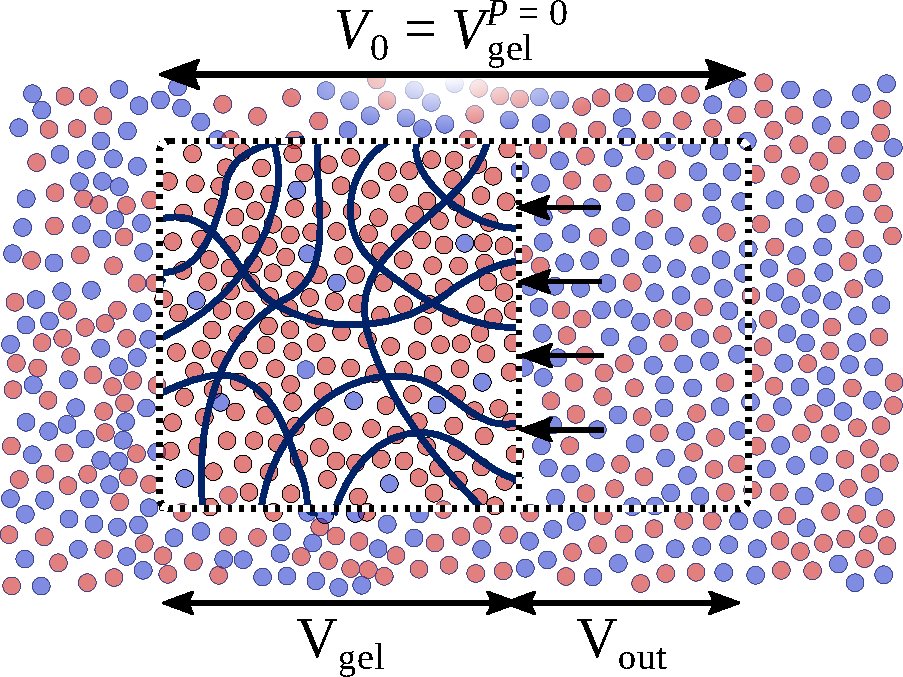
\includegraphics[width=0.5\textwidth]{figures/gc.pdf}}
	\subfloat[Closed system \label{fig: closed}]
	{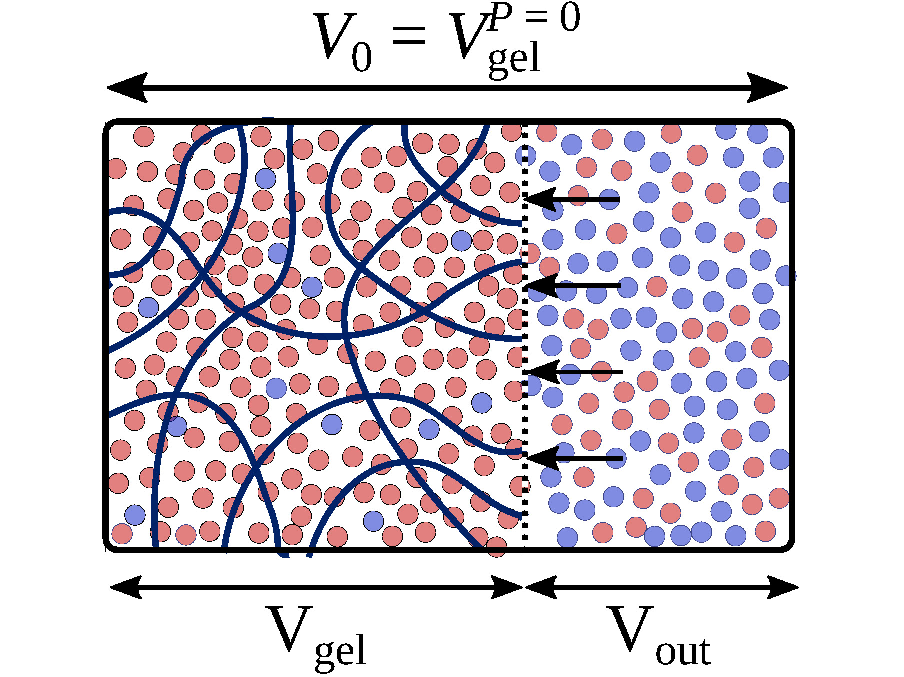
\includegraphics[width=0.5\textwidth]{figures/gibbs.pdf}}}
	
	\caption{The hydrogel compressed in \emph{open} and in \emph{closed} system.
		Red and blue circles represent $\na$ and$\cl$ ions. $V_0$ is the volume which gel has in free swelling equilibrium state.\label{fig:open and closed}}
\end{figure}
%In the case of \emph{open system} the gel is the grand canonical ensemle, as $\mu, V, T = \mbox{Const}$, while the case of \emph{closed system} the gel and the explicit reservoir are a variation of Gibbs ensemble \cite{Panagiotopoulos1988b} performed with constant volume for the both boxes, equal chemical potentials of ion species at constant temperature.

%Unfortunately, there is no universal computationally effective technique to sample pressure difference, volume, and number of particles at the same. 
Mechanical movement and the exchange of ions occur simultaneously in reality; however, we simulate them as alternating in a stop--run mode. 
To sample mechanical properties of the gel and reservoir, we use MD simulation, whereas to sample the ion distribution between the gel and a reservoir, we use MC simulation.
The details of this hybrid MCMD computational technique can be found in our previous studies of polyelectrolytes in open systems \cite{Rud2020, Rud2022, Landsgesel2020a}. 
 
\subsection{Molecular Dynamics}

We model the gel as a network of 16 linear polymer chains, each consisting of 30~monomer units.
These polymer chains are connected to a diamond-like network by eight~crosslinking units.
This means there are $\Ngel=16\cdot30 + 8=488$ gel monomers in the simulation box (see \reffig{fig:diamond}).
The network is put in a simulated cubic box with volume $\Vgel$ with periodic boundary conditions, which virtually emulates an infinite polymer~network.
\begin{figure}[H]
 
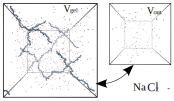
\includegraphics[width=0.7\textwidth]{{figures/simgibbs}.pdf}\caption{Diamond-like network in the simulation box. Color code represents
the individual ion types (red: $\na$, blue: $\cl$)
and the hydrogel (gray: neutral segment ($\AH$), cyan: charged segment
($\A$)). \label{fig:diamond}}
\end{figure}
Each monomer unit of the network carries a negative elementary electric charge.
Except for the gel monomers, the monovalent co- and counter-ions, $\cl$ and $\na$, are present in the simulation box.
The total electric charge of all the particles in the box is zero; therefore the number of $\na$ ions exceeds the number of $\cl$ ions by $\Ngel$.

Each pair of particles interact via the truncated Lennard--Jones interaction potential, which imposes strong repulsion between all particles at short distances:
\begin{equation}
    \begin{split}\label{eq:LJ}
        V_\mathrm{LJ}(r) =
        \begin{cases}
            4 \varepsilon \left( \left(\cfrac{\sigma}{r}\right)^{12}
            - \left(\cfrac{\sigma}{r}\right)^6\right)
            & \mathrm{if~} r < r_\mathrm{cut}\\
            0
            & \mathrm{elsewhere}
        \end{cases},
    \end{split}
\end{equation}
where 
$r$ is the interparticle distance, 
$\sigma = 0.35~\mathrm{nm}$ is a chosen characteristic size of the particles, 
$\varepsilon = \kT$ is the depth of the potential, and 
$r_\mathrm{cut}$ is the cut-off distance beyond which the potential is set zero.

The bonds connecting the gel to a network are modeled using finite extension nonlinear elastic potential (FENE)
\begin{equation}\label{eq:fene}
V_\mathrm{FENE}(r) = -\frac{1}{2} K \Delta r_\mathrm{max}^2\ln \left[ 1 - \left(\frac{r-r_0}{\Delta r_\mathrm{max}} \right)^2 \right ],
\end{equation}
where
$r$ is the distance between the bonded segments,
$K$ is the magnitude of their interaction,
$\Delta r_{\mathrm{max}}$ is the maximal stretching length of the bond, and
$r_0$ is the equilibrium bond length.
For our simulations, we chose $K = 10 \kT/\sigma^{2}$, $\Delta r_{\mathrm{max}} = 2 \sigma$, and $r_0 = 1.0\sigma$~\cite{Jin2007}.



All the charged particles interact via Coulomb electrostatic potential:
\begin{equation}
    V_{\mathrm{EL}}=\lb\kT \cfrac{q_{1}q_{2}}{r},
\end{equation}
where $\lb$ is Bjerrum length---$\lb = 2\sigma = 0.7~\mathrm{nm}$, which corresponds to the  Bjerrum length in water at temperature $T=300~\mathrm{K}$---and $\kB$ is the Botlzman constant.
In that sense, the solvent (water) is accounted for in the model implicitly via setting up dielectric permittivity $\epsilon=80$.

We used the Langevin thermostat, \ie two additional terms for force in the equation of motion were added
\begin{equation}
\mathbf{f}_i =  -\gamma \mathbf{v}_i(t)+\sqrt{2\gamma \kT }\boldsymbol{\eta}_i(t),
\end{equation}
where the first term corresponds to constant friction, with $\gamma$ being a friction coefficient,
 and the second term corresponds to random thermal force, with $\boldsymbol{\eta}_i$ being a normally distributed random vector; $\mathbf{v}_i$ is the velocity of the $i$-th particle (for details see \cite{Grest1986}).

\subsection{Monte Carlo Sampling in an Open System}
The Monte Carlo scheme for sampling the exchange of ions in an \emph{open system} is based on the formula for free energy of grand canonical ensemble $\Omega$
\begin{equation}
    \Omega_{\mathrm{open}}=E-TS+\sum_i\mu_i N_i\label{eq:Omega-GC}
\end{equation}
where $E$ is internal energy, $T$ is temperature, $S$ is entropy, $N_i$ is the number of ions of type $i\in\{\na,\ \cl\}$, and $\mu_i$ is the corresponding chemical potential.

%Our model system represents a finite volume $V$ which exchanges particles with the bath of infinite volume.
%The infinity of the volume means, that the particle exchange between the system and the bath does not influence on the chemical potentials in the bath.
%Such ensemble is called grand canonical ensemble; the free energy in this ensemble, the Landau potential, is
The entropy $S$ is given by the Boltzmann formula~\cite{Nagle2004}
\begin{equation}
    S=\kB\sum_i\ln\frac{\Vgel^{N_i}}{N_i!}\label{eq:entropy}
\end{equation}
%\todo{for partiles without interactions}
which accounts for two contributions:
\begin{enumerate}
    \item The combinatorial entropy $S_{c}=-\kB\sum_i\ln N_i!$, which reflects the freedom of choice among the particles;
    \item The mixing entropy $S_{m}=\kB \sum_i N_i\ln \Vgel$, which reflects the freedom to place the chosen particle randomly within the simulation box. 
\end{enumerate}

$\Vgel$ is the unitless volume, \ie the volume measured in units of $\sigma^3$. 
Thus, the change of free energy associated with an exchange of ion pairs is
\begin{equation}
\Delta\Omega_\mathrm{open}=\kT\ln\prod_i\left(\Vgel^{\xi}\frac{N_i!}{\left(N_i+\xi\right)!}\right)+\xi\sum_i\mu_i+\Delta E
\label{eq: DeltaG GC}
\end{equation}
where $\xi$ is an algebraic number of inserted (or removed) ion pairs; in general, $\xi$ can be any number, but when $\xi = \pm 1$, which corresponds to addition or removal of only one ion pair,  \refeq{eq: DeltaG GC} gets simplified
\begin{equation}
    \Delta\Omega_\mathrm{open}=\kT\ln \Vgel^{2\xi} \prod_i \left(N_i+\theta(\xi)\right)^{-\xi}+\xi\sum_i\mu_i+\Delta E
\label{eq: DeltaG GC_simpl}
\end{equation}
where $\theta$ is the Heaviside function; $\theta(\xi) = 1$ if $\xi=+1$; $\theta(\xi) = 0$ if $\xi=-1$.

The procedure for Monte Carlo sampling is as follows: \cite{Frenlkel2002_book}
\begin{enumerate}
	\item Propose the new configuration of the system by insertion (or deletion) of an ion pair, $\xi=\pm1$;
	\item Accept the new configuration if
	\begin{equation}
        \mathcal{R}^{\xi}<e^{\Delta\Omega_\mathrm{open}/\kT}=\Vgel^{2\xi} \prod_i \left(N_i+\theta(\xi)\right)^{-\xi}e^{\left(\Delta E+\xi\mu\right)/\kT}\label{eq: GC acceptance}
	\end{equation}
	where $\mathcal{R}$ is a uniformly distributed random number in the range between $0$ and $1$;
	\item Then, collect the number of ions, $\Nna$ and $\Ncl$, to the samples array.
\end{enumerate}


\subsection{Monte Carlo Sampling in Closed System}

In the \emph{closed system}, the gel exchanges particles with the explicit finite reservoir box. 
The total number of ion species in both boxes is fixed, whereas the density of ions in the external reservoir is defined by thermodynamic equilibrium between the two subvolumes (see \reffig{fig:open and closed}b. Monte Carlo sampling of the distribution of ions between the subvolumes is performed in a way similar to that described in \cite{Panagiotopoulos1988b, Erdos2020}. 

The free energy of the Gibbs ensemble is a sum of the gel's free energy and that of the external volume.
\begin{equation}
    \Omega_{\mathrm{closed}}=\Egel-T\Sgel + \Eout-T\Sout \label{eq:Omega-GC}
\end{equation}
Using reasoning similar to that of the \emph{open system}, one can derive the change of free energy associated with ion-pair exchange 
\begin{equation}
\Delta \Omega_{\mathrm{closed}} =2 k_B T \ln \left(\frac{\Vgel}{\Vout} \right) ^ {\xi}\prod_i \left(\frac{N_{i}\gel+\theta(\xi)}{N_{i}\out+\theta(-\xi)}\right)^{-\xi} + \Delta \Egel + \Delta \Eout
\end{equation}
where $\xi$ defines the direction of the trial move, so that $\xi = -1$ when an ion pair moves from the gel to the outside volume, and  $\xi = +1$ otherwise; $\Delta \Egel$ and $\Delta \Eout$ are corresponding changes of the potential energy of the gel and the outside volumes, respectively.

Then, the procedure for sampling is the same as that of the \emph{open system}: (1) propose the move of an ion pair; (2) accept a new state if $\mathcal{R}^{\xi}<\exp({\Delta\Omega_\mathrm{closed}/\kT}$); and (3) repeat the procedure until the desired number of samples is reached.

\subsection{Algorithm}
As mentioned above, the whole simulation run consists of MD and MC subsimulations of mechanical movement of the particles and ion exchange. The algorithm follows:
\begin{enumerate}
\item Initiate the systems to simulate: the gel of volume $\Vgel$ and the external solution of volume $\Vout$;
\item Equilibrate the system, interspersing the MD and MC stages;
\item Run the MD subsimulation and collect the observables: pressure in both volumes, $P_\mathrm{gel}$, $P_\mathrm{out}$, and distances between the nodes of the gel network. The latter is needed to estimate the autocorrelation of the MD simulation;
\item Run the MC procedure, simulating ion exchange, and collect the number of ions in both boxes, 
$\Ncl\gel$ and $\Ncl\out$; 
\item Repeat the MD and MC subsimulations until the desired length of sample arrays is reached.
\end{enumerate}


Using the data obtained from simulations, we calculate  
$\cs$, the density of ions in  the outside volume;
$\vgel$, molar volume of the gel, \ie the volume of the gel per one mol of gel segments, $\vgel = \Vgel / \Ngel$;
$\ncl$, the total number of ions in both volumes divided by the total volume of both boxes, $\ncl = \Ncl/\Vbox$; and
$\Pgel$, \emph{partial pressure} of the gel, \ie the pressure that needs to be applied to the gel via a solvent-permeable filter to compress the gel to a specific molar volume.
We obtain the gel partial pressure as the difference between the pressure in the gel and the pressure in the outer volume, $\Pgel=P_\mathrm{gel} - \Pout$.
%$\Pout$, in turn, we obtained from a separate simulation of a reservoir, containing ionic gas in equilibrium with the bath of the same salinity $\cs$. 



The volume $\Vbox$ was chosen to be close to the gel free-swelling equilibrium, that is, to the state where $\Pgel = 0$.
In order to obtain the value $\Vbox$, we perform a set of open system simulations for various $\Vgel$ values.
The value of $\Vgel$ at which $\Pgel$ is closest to zero is chosen as $\Vbox$.
Then, as soon as $\Vbox$ is defined, we compress the gel in the \emph{closed system} with varying values of $\Vgel<\Vbox$ and $\Vout= \Vbox - \Vgel$.

\section{Results and Discussion}

\subsection{Compression in Open System}

Initially, we run a set of simulations modeling the gel compression in an \emph{open system}, \ie in equilibrium with a big bath of certain salinity, $\cs$. 
The simulations are run for a set of different gel volumes, $\Vgel$. 
Each simulation returns the averaged values of pressures, $P_\mathrm{gel}$, and the number of $\cl$ ions present in the simulation box, $\Ncl\gel$. 

The dependencies of $\Pgel$ on $\Vgel$ for the \emph{open system} for a set of various salinities are presented
in Figure \ref{fig: PV and CV}a as solid lines. 
For example, the blue solid line illustrates the compression (or swelling) of the gel in equilibrium with a reservoir of salinity $\cs=0.063$ mol/L. 
The points where the pressure equals zero, $\Pgel=0$, (indicated by filled circles) are the gel \emph{free-swelling equilibrium} states.
These states are characterized by the corresponding molar volume of the gel, $\Vgel^0$, and the amount of ions in gel \{$\Nna^0$, $\Ncl^0$\} 
(Index ``0'' stands for zero bar applied pressure).
The \emph{free-swelling equilibrium} state positions shift towards smaller volumes with increased salinity. 
In general, increased salinity shifts all the $\Pgel(V)$ curves towards smaller volumes.
This effect is well known and is typical for all branched \emph{strong} polyelectrolytes. 
It is caused by the decrease of ion osmotic pressure and by the screening of electrostatic interactions \cite{Zhulina2000, Landsgesel2020a}.
(The salinity dependence on the size of a \emph{weak} polyelectrolyte gel is in general non-monotonic. We discuss this in \cite{Rud2018}.)
\begin{figure}[H]
	\begin{adjustwidth}{-\extralength}{0cm}
	\centering
	{\captionsetup{position=bottom,justification=centering}
	\subfloat[Gel partial pressure vs. gel molar volume \label{fig: PV}]
		{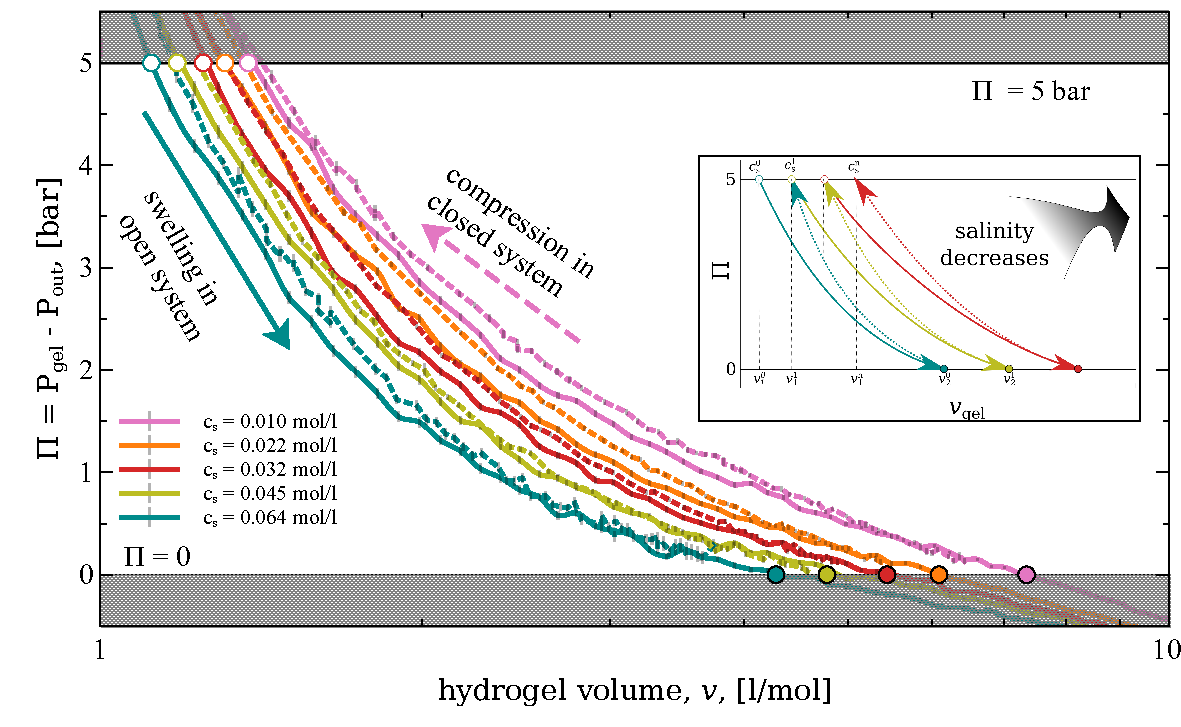
\includegraphics[width=0.65\textwidth]{figures/fig_PV_pub.pdf}}
	\hspace{0.02\textwidth}
	\subfloat[Supernate salinity vs. gel molar volume\label{fig: CV}]
		{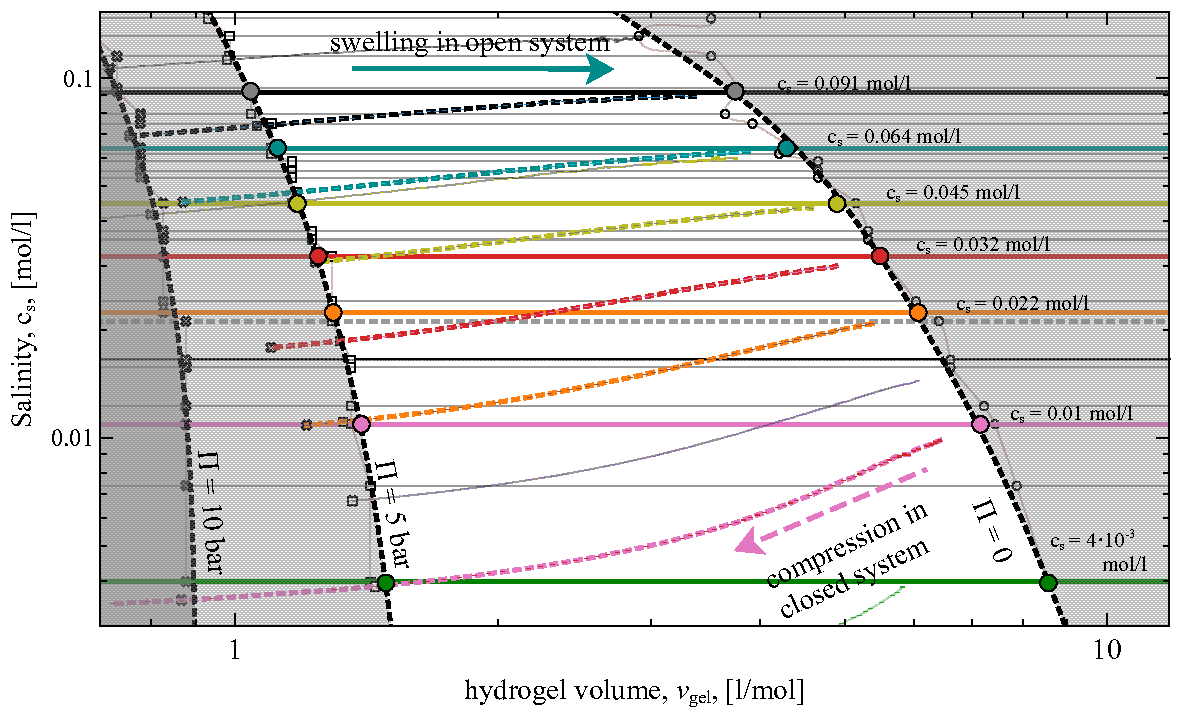
\includegraphics[width=0.65\textwidth]{figures/fig_CV_pub.pdf}}	}\end{adjustwidth}
	\caption{
	Compression of the gel in the \emph{open system} (solid lines) and in the \emph{closed system} (dotted lines). 
	Each solid curve corresponds to different salinity of the reservoir $\cs$ (see legend).
	The shaded areas limit the states with applied pressure below zero and above 5 bar.\label{fig: PV and CV}}

\end{figure}



\subsection{Compression in Closed System}
The simulations in the \emph{closed systems} start from the $\Vgel^0$ and \{$\Nna^0$, $\Ncl^0$\} values
obtained from the corresponding \emph{open system} simulations.
The simulation of gel compression in a closed volume, $\Vbox$, starts at the point $\Vbox = \Vgel^0$
and ion content $\Ncl^0$ for $\cl$ ions. The number of $\na$ ions neutralizes the system, $\Nna^0 = $$\Ncl^0 + \Ngel$.

We prepare two systems: one for simulation of the gel at the volume $\Vgel$
and the other for simulation of the supernatant solution at the volume $\Vout = \Vbox - \Vgel$.
Note that the number of $\Ncl^0$ and $\Nna^0$ ions  %Please ensure meaning has been retained.
are shared by the two volumes. 

The processes of gel compression in the \emph{closed system} is depicted in Figure~\ref{fig: PV and CV}a as dotted lines.
In this plot, for example, the blue dotted line illustrates the compression of the gel equilibrated with solution with salinity $\cs=0.063$ mol/L at the volume at which the gel has zero pressure. 
The volume values $\Vgel$ and $\Vout$ are comparable in the \emph{closed system} case.
Therefore, gel compression decreases the salinity in the supernate, $\cs$. 
This dependence is illustrated in \reffig{fig: PV and CV}b, where the same swelling/compression processes are displayed in different coordinates: \ie salinity of the supernate versus the gel molar volume, $\cs(\Vgel)$.
In these coordinates, all the open-system compressions show up as horizontal lines, which reflects the constant salinity, whereas the compressions in the closed system demonstrate the change of $\cs$ from $\cs^{0}=0.063$ at the zero-pressure $\Pgel$ to $\cs^{5}=0.045$~mol/L at $P\gel=5$ bar (index ``5'' stands for 5 bar). 

Although the salinity during compression in the \emph{open system} remains constant, the number of ions in the compressed subsystem (\ie in the volume where the gel is compressed (or swells)) changes.
Here, the compression volume $\Vbox$ is the volume of the \emph{free-swelling equilibrium} state of the gel, $\Vbox = \Vgel^0$.
Figure \ref{fig: NV and CN}a shows number of $\cl$ ions in the volume $\Vbox$ per unit volume, $\ncl =$ $\Ncl/\Vbox$, as a function of the gel molar volume. 
The depicted values can be considered as the average density of $\cl$ ions in the compression volume $\Vbox$. 

The $\ncl$-$\Vgel$ dependencies look like horizontal lines in the case of \emph{closed system} compression,
whereas $\ncl$ increases with $\Vgel$ during the compression in the \emph{open system} case. 
This implies, that the compression of the gel in the \emph{open system} pulls out the ions from the bath to the compression volume, $\Vbox$. 
And vice versa, the swelling of the gel pushes ions out to the bath.
\begin{figure}[H]
\begin{adjustwidth}{-\extralength}{0cm}
{\captionsetup{position=bottom,justification=centering}
\subfloat[Pressure vs. gel molar volume \label{fig: NV}]
{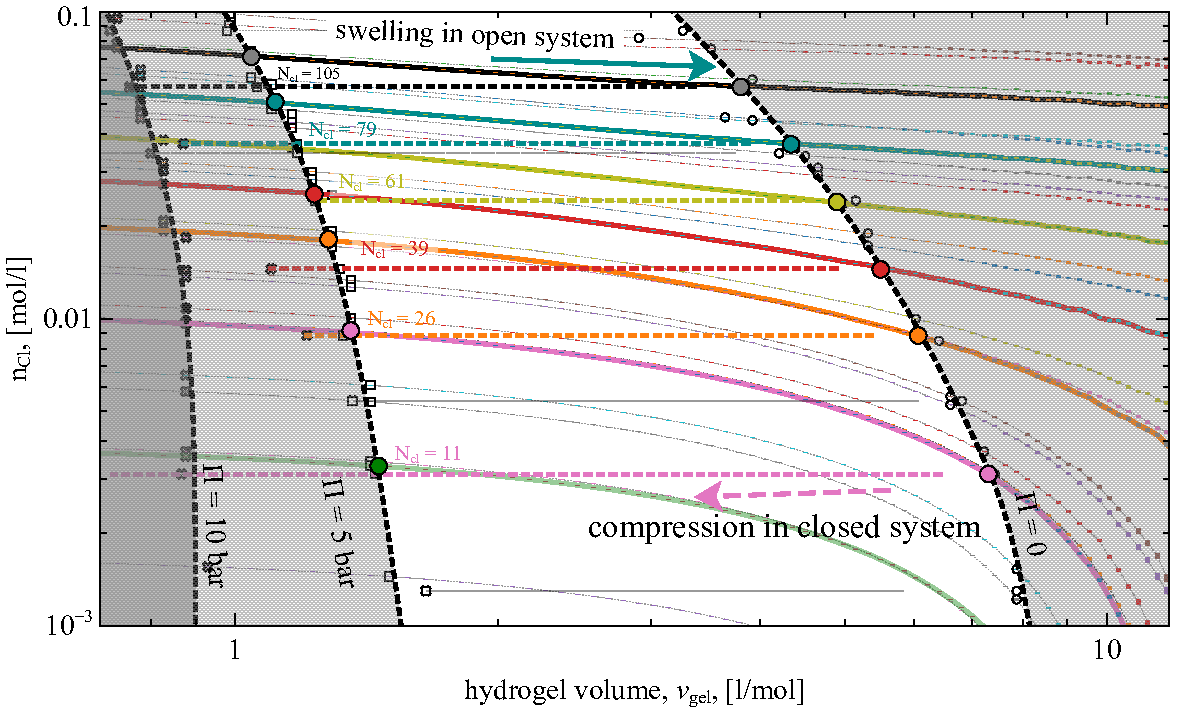
\includegraphics[width=0.65\textwidth]{figures/fig_NV_pub.pdf}}
\hspace{0.02\textwidth}
\subfloat[Salinity vs. gel molar volume\label{fig: CN}]
{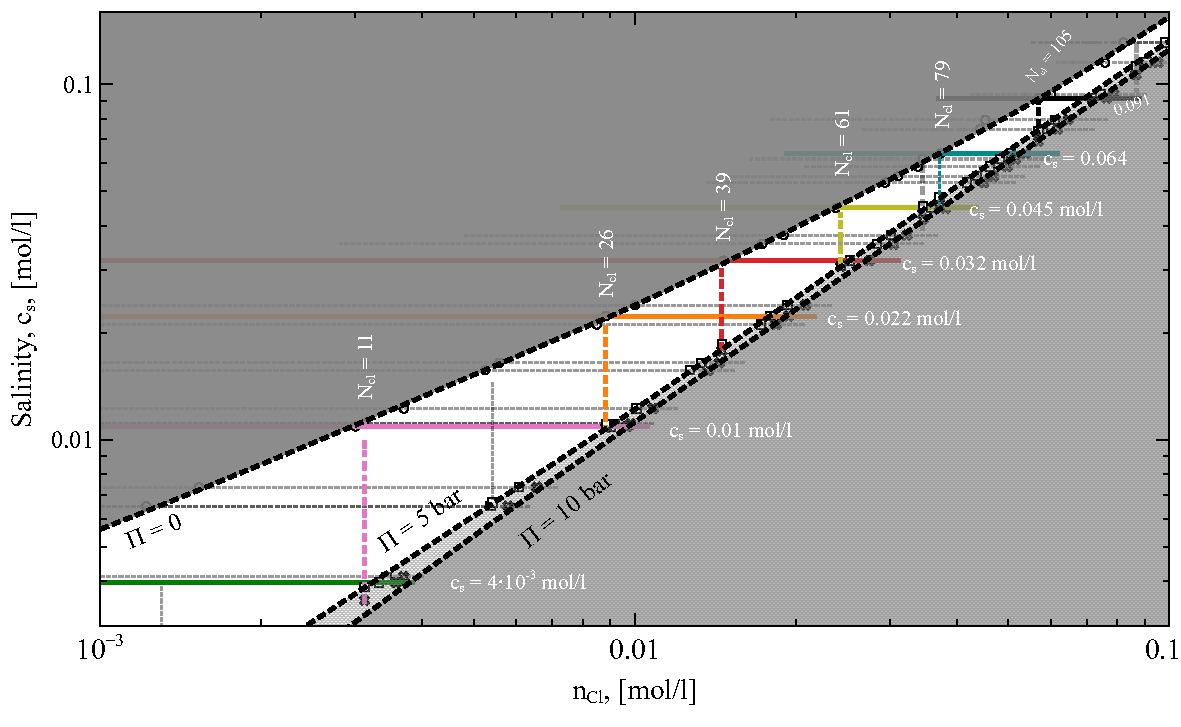
\includegraphics[width=0.65\textwidth]{figures/fig_NVbox_mu_pub.pdf}}}\end{adjustwidth}
\caption{The compression of the gel in \emph{open system} (solid lines) and in \emph{closed system} (dotted lines). 
Shadowed area limit the states with applied pressure below zero and above 5 bar.
The values $N_\cl$ are the virtual numbers of present $\cl$ ions in \emph{closed system} simulation boxes.
\label{fig: NV and CN}}

%\todoi{Replace y-axis labels by $\ncl$}
\end{figure}
Finally, the same processes are depicted in Figure \ref{fig: NV and CN}b in coordinates $\ncl$---$\cs$. 
In these coordinates, both ways of the compression, in \emph{open} and in \emph{closed} systems, appear as straight vertical and horizontal lines correspondingly. 

In our study, we modeled the compression of the gel in equilibrium with reservoirs of 40 different salinities, ranging from 0.001 to 0.5 mol/L. 
The \emph{open system} compressions resulted in defined free-swelling equilibrium states,
which we used as the initial conditions for the respective compressions in the \emph{closed system}. 
All the corresponding dependencies are depicted in Figures~\ref{fig: PV and CV} and \ref{fig: NV and CN} as thin grey dashed lines (some of them are highlighted and colored).
The states corresponding to $P^{gel}=0$, 5, and 10 bar pressures are marked by open circles, squares, and crosses, respectively. 
The non-shaded areas in the figures highlight the states in which the gel partial pressure ranges between the experimentally relevant values of 0 and 5 bar.

\subsection{Desalination Scheme}
It follows that compression of the gel in the \emph{closed system} affects the salinity, whereas compression in the \emph{open system} affects the number of ions in the gel subsystem. 
Here, we show how to employ these phenomena for water desalination. 
The highlighted colored lines on the plots in Figures \ref{fig: PV and CV} and \ref{fig: NV and CN} form a sequence of gel swellings and compressions, following one another and corresponding to  \emph{open} and \emph{closed} systems. 
This sequence forms the water desalination process.
Starting from swelling the gel in the \emph{open system} at high salinity ($\cs=0.091$ mol/L, solid black line), the gel is compressed in the \emph{closed system} until the pressure reaches 5 bar (dashed black line). 
Then, the same gel swells in a reservoir with slightly lower salinity in the \emph{open system} (\ie $\cs=0.064$ mol/L, light blue line). 
After swelling, the gel is compressed again with 5 bar pressure in the \emph{closed system} (dashed light blue line).  
Then, the gel swells in a reservoir of even smaller salinity ($\cs=0.045$ mol/L, solid yellow line), and so on. 
This chain of alternating swellings and compressions ends up when salinity is equal to $\cs=4\times10^{-3}$ mol/L after compression in the \emph{closed system} (dashed magenta line).

The plots in Figures \ref{fig: PV and CV} and \ref{fig: NV and CN} depict the whole process in all possible coordinate representations.
In all plots, the lines corresponding to sequential swellings and compressions during the whole desalination process resemble a 'pathway'.
In particular, the desalination process depicted in Figure~\ref{fig: NV and CN}b resembles a staircase,
where the \emph{open system} processes are horizontal lines and the \emph{closed system} processes are vertical lines.

%\begin{enumerate}
%    \item as gel partial pressure versus gel molar volume, $\Pgel(\Vgel)$ (\ref{fig: PV}), 
%    \item as supernatant salinity versus gel molar volume, $\cs(\Vgel)$ (\ref{fig: CV}),
%    \item the amount of $\cl$ ions in a compression volume versus gel volume, $\ncl(\Vgel)$ (\ref{fig: NV}), 
%    \item $\ncl$ as function of supernatant salinity.
%\end{enumerate}




%Then we repeat the simulation of hydrogel swelling in open system but setting as a salinity of the reservoir the new, obtained from the previous process, value $\cs=$ 0.045 mol/L. 
%Again, as soon as we obtain the free swelling equilibrium state (at new salinity), with corresponding new values of $V\gel$ and $\ncl$, we start simulating the compression in closed system. Now the salinity changes again, decreasing from 0.045 to 0.031 mol/L (at 5 bar). 
%These two processes are depicted by solid and dotted yellow lines in Figure~\ref{fig:fig_PV}.
%The Figure shows also the repetition of this procedure three more times until the salinity reaches the value $\cs=0.01$ mol/L. 
%The last dashed magenta line shows the compression in closed system which ends up with $\cs=4\cdot10^{-4}$ mol/L. 
%Schematically this process is depicted in the inset to the plot.



%The same process is depicted on Figure~\ref{fig:fig_CV} but in different coordinates: salinity versus volume. 
%In this coordinates the swelling in open system appear to be horizontal line, since the salinity in this process is constant. 
%Again we start from swelling in open system untill the gel reaches its free swelling equilibrium (solid blue line).
%Then the gel is compressed in closed system (dashed blue line), ending up in a state with applied to the gel pressure 5 bar. 
%In this process the surrounding solution salinitiy changes from 0.064 to 0.045 mol/L.
%Then the gel again swells in open system, but at new salinity. 

\subsection{The Efficiency of Desalination}
The theoretical minimum specific energy for seawater desalination ($\cs\simeq0.6$ mol/L for pure NaCl) is $\sim$$3.9$ kJ/L (1.1 kWh/m$^3$) for 50\% recovery \cite{Wang_2020}.
This value is calculated as~follows
\begin{equation}
W_{\mathrm{id}}=2RT\left(\frac{c_{f}}{R_{w}}\ln\frac{c_{b}}{c_{f}}-c_{p}\ln\frac{c_{b}}{c_{p}}\right)
\label{eq:SEC}
\end{equation}
where $R$ is the universal gas constant, $c_{f}$ is the salinity of the feedwater, $c_p$ is the salinity of the product water, $c_b$ is the salinity of the brine, which necessarily appears in any desalination process, and
$R_{w}$ is the recovery ratio, \ie the ratio of the volume of water produced and the feedwater volume. A 50\% recovery ratio means that one part feedwater divides into two equal volume solutions of product water and brine.
Of course, a significant amount of additional energy is required to operate the system \cite{Kim_2019}.
It has been reported that the specific energy consumption (SEC) of reverse osmosis (RO) is 2.5--4.0 kWh/m3 (9.0--14.4 kJ/L), which is significantly higher than its minimum specific energy.
The SEC of a real-scale RO plant is even higher, approximately 3.5--4.5~kWh/m$^{3}$ (12.6--16.2~kJ/L), including pre-treatment and post-treatment processes~\cite{Kim_2018}.
%Because of the inherent high energy requirement for RO desalination, seawater is not commonly utilized over traditional surface water.

To compare the efficiency of the desalination process presented in Figures \ref{fig: PV and CV} and \ref{fig: NV and CN} with provided values, we collect the corresponding data in Table~\ref{tab: table}.
The presented desalination process is a cascade of six swellings in an open system at six different (constant) salinities $\cs$, each followed by six compressions in a closed system at six different (constant) $\ncl$.
Each swelling and compression process is presented as a row in Table~\ref{tab: table}, which is colored by matching the lines in the figures.
The first column of the table contains values for $\cs^0$ and $\cs^5$, which stand for the supernate salinity at 0 and 5 bar compression, respectively; in an open system, supernate salinity does not change, so $\cs^0$ and $\cs^5$ are represented by a single number.
The second column contains values of $n^0$ and $n^5$, which stand for the number of $\cl$ ions in compression volume $\Vbox$ at 0 and 5 bar pressure, respectively, (divided by $\Vbox$).
The number of ions does not change in closed system compression; thus, $n^0$ and $n^5$ are the same in the corresponding rows.
The third column shows the change of the gel volume in the corresponding process, $\Delta v$.
The fourth column contains the work needed for compression in the corresponding process per volume of extracted solution.
This value is obtained as the numerical integration of corresponding $\Pgel(\Vgel)$ dependence \citep{Atkins}
\begin{equation}
W = \frac{\int_{v^0}^{v^5} \Pgel d\Vgel}{\Delta v}
\end{equation}

In this column, we present the absolute values of the work,
whereas one should keep in mind that compression implies that the work is done by external force, and swelling implies that the work is done by the gel.

For comparison with ideal desalination process efficiency, the fifth column provides values for ideal specific energy consumption, $W^\text{id}$, which are calculated employing \refeq{eq:SEC}, for the concentrations of feed, product, and brine solutions, $\cs^f$,  $\cs^p$, $\cs^b$, respectively, as indicated by curly brackets.
For example, with $\cs^f=44.91$, $\cs^p=31.93$, and $\cs^b = 63.93$~mmol/L, (fifth, seventh, and third rows of the table), one can imagine the following desalination~process
\begin{enumerate}
\item First, the gel equilibrates with the feed solution and is compressed in the \emph{closed system}.
The gel volume decreases by $\Delta v^p = 3.69$ liters, and the salinity of the supernate decreases from $\cs^f$ to $\cs^p$.
The volume of the product solution is $\Delta v^p$.
\item The squeezed gel is put back into the feed solution and is equilibrated there under pressure, so it does not swell.
\item After equilibration, the gel swells in the \emph{closed system}, so the salinity of the external solution increases to the value $\cs^b$.
\item Finally, the gel is taken out and compressed at 5 bar pressure in the \emph{open system} in equilibrium with the brine bath.
The change of the gel volume in this process is $\Delta v^b = 3.26$ L/mol, which equals the volume of the produced brine.
\end{enumerate}


\begin{table}[H]
\caption{Estimates of  %MDPI: Please confirm if the format of the table should be retained, e.g., the color of the font, the text direction, vertical line
% Oleg Rud: Confirm the colors and the directions of the table must retain
desalination efficiency. All units are calculated per one mol of gel segments. Values in brackets correspond to crossection of `red' and `orange' lines on the plots in Figures \ref{fig: PV and CV} and \ref{fig: NV and CN}.
\label{tab: table}}

\begin{adjustwidth}{-\extralength}{0cm}

		\newcolumntype{C}{>{\centering\arraybackslash}X}
\begin{tabularx}{1\fulllength}{@{\extracolsep{\fill}}ll|lc|c|l|ll}
\noalign{\hrule height 1pt}
\multicolumn{1}{l|}{\textbf{\boldmath{$c_{s}^{0}$}, mM}} & \textbf{\boldmath{$c_{s}^{5}$}, mM} & \multicolumn{1}{l|}{\textbf{\boldmath{$n_{\cl}^{0}$}, mM}} & \textbf{\boldmath{$n_{\cl}^{5}$}, mM} & \textbf{\boldmath{$\Delta \Vgel$}, L} & \textbf{\boldmath{$|W$}\textbar , J/L} & \multicolumn{2}{c}{\textbf{\boldmath{$W^{id}$}, J/L}}\tabularnewline
 
\noalign{\hrule height 0.5pt} 
\multirow{2}{*}{{\small{}$91.47$}} & \multirow{2}{*}{} & \multicolumn{2}{l|}{{\small{}$57.08\pm0.122\enskip\longrightarrow$}} & \multirow{2}{*}{{\small{}2.74}} & \multirow{2}{*}{{\small{}$95.4\pm1.9$}} &  & \multirow{2}{*}{}\tabularnewline
 &  & \multicolumn{2}{r|}{{\small{}$71.75\pm0.024$}} &  &  & \multirow{8}{*}{{\small{}\hspace{-1em}}\textcolor{teal}{\small{}$\left.\begin{array}{l}
\\
\\
\\
\\
\\
\\
\\
\\
\end{array}\right\rbrace $$\rotatebox{90}{\hspace{-5em}{\color{teal}\ensuremath{\begin{array}{cc}
W^{id}= & 52.9\\
W^{\mathrm{sim}}= & 202.8\pm3.2\\
R_{w}= & 0.54
\end{array}}}}$}} & \tabularnewline
\cline{1-6} \cline{2-6} \cline{3-6} \cline{4-6} \cline{5-6} \cline{6-6} 
\multicolumn{2}{l|}{{\small{}$89.41\pm0.23\enskip\longrightarrow$}} & \multirow{2}{*}{{\small{}56.90}} & \multirow{2}{*}{} & \multirow{2}{*}{{\small{}2.72}} & \multirow{2}{*}{{\small{}$109.1\pm1.7$}} &  & \multirow{2}{*}{}\tabularnewline
\multicolumn{2}{r|}{{\small{}$73.63\pm0.03$}} &  &  &  &  &  & \tabularnewline
\cline{1-6} \cline{2-6} \cline{3-6} \cline{4-6} \cline{5-6} \cline{6-6} 
\multirow{2}{*}{\textcolor{teal}{\small{}63.93}} & \multirow{2}{*}{} & \multicolumn{2}{l|}{\textcolor{teal}{\small{}$37.28\pm0.08\enskip\longrightarrow$}} & \multirow{2}{*}{\textcolor{teal}{\small{}3.26}} & \multirow{2}{*}{\textcolor{teal}{\small{}$100.9\pm1.7$}} &  & \tabularnewline
 &  & \multicolumn{2}{r|}{\textcolor{teal}{\small{}$50.579\pm0.013$}} &  &  &  & \multirow{8}{*}{{\small{}\hspace{-1em}}\textcolor{olive}{\small{}$\left.\begin{array}{l}
\\
\\
\\
\\
\\
\\
\\
\\
\end{array}\right\rbrace $$\rotatebox{90}{\hspace{-5em}\ensuremath{\begin{array}{cc}
W^{id}= & 38.2\\
W^{\mathrm{sim}}= & 207.3\pm2.2\\
R_{w}= & 0.53
\end{array}}}$}}\tabularnewline
\cline{1-6} \cline{2-6} \cline{3-6} \cline{4-6} \cline{5-6} \cline{6-6} 
\multicolumn{2}{l|}{\textcolor{teal}{\small{}$62.05\pm0.15\enskip\longrightarrow$}} & \multirow{2}{*}{\textcolor{teal}{\small{}37.17}} & \multirow{2}{*}{} & \multirow{2}{*}{\textcolor{teal}{\small{}3.18}} & \multirow{2}{*}{\textcolor{teal}{\small{}$107.4\pm1.4$}} &  & \tabularnewline
\multicolumn{2}{r|}{\textcolor{teal}{\small{}$48.21\pm0.02$}} &  &  &  &  &  & \tabularnewline
\cline{1-6} \cline{2-6} \cline{3-6} \cline{4-6} \cline{5-6} \cline{6-6} 
\multirow{2}{*}{\textcolor{olive}{\small{}44.91}} & \multirow{2}{*}{} & \multicolumn{2}{l|}{\textcolor{olive}{\small{}$23.75\pm0.06\enskip\longrightarrow$}} & \multirow{2}{*}{\textcolor{olive}{\small{}3.82}} & \multirow{2}{*}{\textcolor{olive}{\small{}$106.7\pm1.5$}} &  & \tabularnewline
 &  & \multicolumn{2}{r|}{\textcolor{olive}{\small{}$35.911\pm0.010$}} &  &  & \multirow{8}{*}{{\small{}\hspace{-1em}}\textcolor{red}{\small{}$\left.\begin{array}{l}
\\
\\
\\
\\
\\
\\
\\
\\
\\
\end{array}\right\rbrace \rotatebox{90}{\hspace{-5em}\ensuremath{\begin{array}{cc}
W^{\mathrm{id}}= & 43.8\ {\color{red}{\scriptstyle (41.0)}}\\
W^{\mathrm{sim}}= & 222.3\pm2.5\\
R_{w}= & 0.52\ {\scriptstyle (0.46)}
\end{array}}}$}} & \tabularnewline
\cline{1-6} \cline{2-6} \cline{3-6} \cline{4-6} \cline{5-6} \cline{6-6} 
\multicolumn{2}{l|}{\textcolor{olive}{\small{}$43.46\pm0.12\enskip\longrightarrow$}} & \multirow{2}{*}{\textcolor{olive}{\small{}24.27}} & \multirow{2}{*}{} & \multirow{2}{*}{\textcolor{olive}{\small{}3.91}} & \multirow{2}{*}{\textcolor{olive}{\small{}$106.4\pm1.1$}} &  & \tabularnewline
\multicolumn{2}{r|}{\textcolor{olive}{\small{}$30.795\pm0.008$}} &  &  &  &  &  & \tabularnewline
\cline{1-6} \cline{2-6} \cline{3-6} \cline{4-6} \cline{5-6} \cline{6-6} 
\multirow{2}{*}{\textcolor{red}{\small{}31.93}} & \multirow{2}{*}{} & \multicolumn{2}{l|}{\textcolor{red}{\small{}$14.66\pm0.04\enskip\longrightarrow$}} & \multirow{2}{*}{\textcolor{red}{\small{}4.20}} & \multirow{2}{*}{\textcolor{red}{\small{}$107.9\pm1.4$}} &  & \tabularnewline
 &  & \multicolumn{2}{r|}{\textcolor{red}{\small{}$25.297\pm0.006$}} &  &  &  & \multirow{8}{*}{{\small{}\hspace{-1em}}\textcolor{orange}{\small{}$\left.\begin{array}{l}
\\
\\
\\
\\
\\
\\
\\
\\
\\
\end{array}\right\rbrace \rotatebox{90}{\hspace{-5em}\ensuremath{\begin{array}{cc}
W^{id}= & 66.6\ {\scriptstyle (22.0)}\\
W^{\mathrm{sim}}= & 218.7\pm2.2\\
R_{w}= & 0.53\ {\scriptstyle (0.49)}
\end{array}}}$}}\tabularnewline
\cline{1-6} \cline{2-6} \cline{3-6} \cline{4-6} \cline{5-6} \cline{6-6} 
\multicolumn{2}{l|}{\textcolor{red}{\small{}$30.03\pm0.08\enskip\longrightarrow$}} & \multirow{2}{*}{\textcolor{red}{\small{}14.55}} & \multirow{2}{*}{} & \multirow{2}{*}{\textcolor{red}{\small{}$\begin{array}{c}
4.17\\
{\scriptstyle (3.22)}
\end{array}$}} & \multirow{2}{*}{\textcolor{red}{\small{}$\begin{array}{c}
115.6\pm0.9\\
{\scriptstyle (57.3)}
\end{array}$}} &  & \tabularnewline
\multicolumn{2}{r|}{\textcolor{red}{\small{}$\begin{array}{c}
18.585\pm0.004\,\\
{\scriptstyle (22.32)}
\end{array}$}} &  &  &  &  &  & \tabularnewline
\cline{1-6} \cline{2-6} \cline{3-6} \cline{4-6} \cline{5-6} \cline{6-6} 
\multirow{2}{*}{\textcolor{orange}{\small{}22.30}} & \multirow{2}{*}{} & \multicolumn{2}{l|}{\textcolor{orange}{\small{}$8.84\pm0.03\enskip\longrightarrow$}} & \multirow{2}{*}{\textcolor{orange}{\small{}$\begin{array}{c}
4.75\\
{\scriptstyle (3.76)}
\end{array}$}} & \multirow{2}{*}{\textcolor{orange}{\small{}$\begin{array}{c}
108.1\pm1.3\\
{\scriptstyle (68.3)}
\end{array}$}} &  & \tabularnewline
 &  & \multicolumn{2}{r|}{\textcolor{orange}{\small{}$\begin{array}{c}
\text{17.945}\pm\text{0.004}\\
{\scriptstyle (14.56)}
\end{array}$}} &  &  & \multirow{7}{*}{{\small{}\hspace{-1em}}\textcolor{magenta}{\small{}$\left.\begin{array}{l}
\\
\\
\\
\\
\\
\\
\\
\end{array}\right\rbrace \rotatebox{90}{\hspace{-5em}\ensuremath{\begin{array}{cc}
W^{id}= & 69.7\\
W^{\mathrm{sim}}= & 227.5\pm2.3\\
R_{w}= & 0.55
\end{array}}}$}} & \\[1ex]
\cline{1-6} \cline{2-6} \cline{3-6} \cline{4-6} \cline{5-6} \cline{6-6} 
\multicolumn{2}{l|}{\textcolor{orange}{\small{}$20.74\pm0.06\enskip\longrightarrow$}} & \multirow{2}{*}{\textcolor{orange}{\small{}8.83}} & \multirow{2}{*}{} & \multirow{2}{*}{\textcolor{orange}{\small{}$4.71$}} & \multirow{2}{*}{\textcolor{orange}{\small{}$110.8\pm0.8$}} &  & \tabularnewline
\multicolumn{2}{r|}{\textcolor{orange}{\small{}$11.082\pm0.002$}} &  &  &  &  &  & \tabularnewline
\cline{1-6} \cline{2-6} \cline{3-6} \cline{4-6} \cline{5-6} \cline{6-6} 
\multirow{2}{*}{\textcolor{magenta}{\small{}10.90}} & \multirow{2}{*}{} & \multicolumn{2}{l|}{\textcolor{magenta}{\small{}$3.00\pm0.01\enskip\longrightarrow$}} & \multirow{2}{*}{\textcolor{magenta}{\small{}6.08}} & \multirow{2}{*}{\textcolor{magenta}{\small{}$106.9\pm1.1$}} &  & \tabularnewline
 &  & \multicolumn{2}{r|}{\textcolor{magenta}{\small{}9.011$\pm$0.002}} &  &  &  & \tabularnewline
\cline{1-6} \cline{2-6} \cline{3-6} \cline{4-6} \cline{5-6} \cline{6-6} 
\multicolumn{2}{l|}{\textcolor{magenta}{\small{}$9.83\pm0.05\enskip\longrightarrow$}} & \multirow{2}{*}{\textcolor{magenta}{\small{}3.12}} & \multirow{2}{*}{} & \multirow{2}{*}{\textcolor{magenta}{\small{}5.78}} & \multirow{2}{*}{\textcolor{magenta}{\small{}$119.4\pm1.0$}} &  & \tabularnewline
\multicolumn{2}{r|}{\textcolor{magenta}{\small{}$3.862\pm0.001$}} &  &  &  &  &  & \\[2ex]
\noalign{\hrule height 1pt}
\end{tabularx}
\end{adjustwidth}
\end{table}

Thus, the recovery ratio $R_w = \Delta v^p / (\Delta v^p + \Delta v^b) \simeq $ 0.53 and the theoretical minimum specific energy of the desalination process with corresponding $\cs^f$, $\cs^p,$ and $\cs^b$ is $W^{id} =$ 38.2~J/L (\refeq{eq:SEC}).

The estimated $W^{id}$ values are provided in the fifth column of the table for five triplets of $\cs^f$, $\cs^p$,$\cs^b$ values.
In the same column, we provide $W_{\mathrm{sim}}$---the specific energy consumption calculated by a numerical integration of $\Pgel(\Vgel)$ dependencies. 
The provided values  $W_{\mathrm{sim}}$ are the sum of energies needed for corresponding compression processes, \ie in the \emph{closed} and \emph{open} systems.
The values $R_w$, which are also provided in fifth column, are the corresponding recovery ratios.

The ratio between $W_{\mathrm{sim}}$ and $W_{\mathrm{id}}$ ranges from 3.26 to 5.43, which is comparable to that of RO.
Note that when calculating $W_{\mathrm{sim}}$, we accounted for only the work done on the gel during compression, whereas the work done by the gel itself during swelling was not taken into account. 
The process that accounts for energy recovery was described in our previous studies \cite{Prokacheva2021, Rud2018} 

\subsection{Study Limitations}
Like other simulation-based studies, our research has limited validity, primarily resulting from the simplifications applied in the used model.
For example, our coarse-grained model cannot differentiate polystyrene sulphonate gel from other strong polyacidic gels.
However, these limitations are also the advantage of our model, because the results of our study
can be applied to similar systems, including polybasic gels with all the charges~reversed.

\subsection{Implications and Future Perspectives}
We are aware that the concept introduced in this simulation study needs to be experimentally verified.
Therefore, in the future, we want to focus on experimental aspects of desalination based on polyacidic gel compression. 

\section{Conclusions}
\textls[-5]{We have modeled compression of a polyelectrolyte gel in thermodynamic equilibrium with a supernatant aqueous solution of limited amount.
We have shown that compression of the gel decreases the supernatant salinity.
We employed this phenomenon to model water desalination.
The desalination was done as a sequential combination of two processes:
(1) swelling of the gel in an \emph{open system}, exchanging ions with a large reservoir at constant salinity;
(2) compression of the gel in a \emph{closed system}, during which the gel exchanges ions with a small reservoir, affecting its salinity.
We estimated the energy consumption needed for producing one liter of potable water from brine and have shown that the proposed gel compression method may compete with modern desalination~technologies. %MDPI: we noticed that the supplementary file has been uploaded in submitting system. please confirm if there is a supplementary, if so, please cite it in main text and add section of supplementary materils “\supplementary{The following are available at \linksupplementary{s1}, Figure S1: title, Table S1: title, Video S1: title.} ”. Please note that the reference in supplementary should be also included in mian text.
% Oleg Rud: There is no need of supplementary materials anymore, since we added the method description into the main text.
}


%%%%%%%%%%%%%%%%%%%%%%%%%%%%%%%%%%%%%%%%%%
\vspace{6pt} 

%%%%%%%%%%%%%%%%%%%%%%%%%%%%%%%%%%%%%%%%%%
%% optional
%\supplementary{The following supporting information can be downloaded at:  \linksupplementary{s1}, Figure S1: title; Table S1: title; Video S1: title.}

% Only for the journal Methods and Protocols:
% If you wish to submit a video article, please do so with any other supplementary material.
% \supplementary{The following supporting information can be downloaded at: \linksupplementary{s1}, Figure S1: title; Table S1: title; Video S1: title. A supporting video article is available at doi: link.}

%%%%%%%%%%%%%%%%%%%%%%%%%%%%%%%%%%%%%%%%%%
\authorcontributions{Conceptualization, O.V.R.; methodology, M.L.; software, M.L.; validation, M.L., L.N., and O.V.R.; formal analysis, L.N.; data curation, M.L.; writing---original draft preparation, O.V.R.; writing---review and editing, L.N. All authors have read and agreed to the published version of the manuscript.
%All authors have read and agreed to the published version of the manuscript.', please turn to the  \href{http://img.mdpi.org/data/contributor-role-instruction.pdf}{CRediT taxonomy} for the term explanation. Authorship must be limited to those who have contributed substantially to the work~reported.
}

\funding{``This research was funded by Czech Science Foundation grant number 19-17847Y'' and government of the Russian Federation grant number 14.W03.31.0022. }

%\institutionalreview{\hl{~}}%MDPI: In this section, please add the Institutional Review Board Statement and approval number for studies involving humans or animals. Please note that the Editorial Office might ask you for further information. Please add ``The study was conducted according to the guidelines of the Declaration of Helsinki, and approved by the Institutional Review Board (or Ethics Committee) of NAME OF INSTITUTE (protocol code XXX and date of approval).'' OR ``Ethical review and approval were waived for this study, due to REASON (please provide a detailed justification).'' OR ``Not applicable'' for studies not involving humans or animals. You might also choose to exclude this statement if the study did not involve humans or animals.

%\informedconsent{\hl{~}}%MDPI: Any research article describing a study involving humans should contain this statement. Please add ``Informed consent was obtained from all subjects involved in the study.'' OR ``Patient consent was waived due to REASON (please provide a detailed justification).'' OR ``Not applicable'' for studies not involving humans. You might also choose to exclude this statement if the study did not involve humans. Written informed consent for publication must be obtained from participating patients who can be identified (including by the patients themselves). Please state ``Written informed consent has been obtained from the patient(s) to publish this paper'' if applicable.

%\dataavailability{\hl{~}} %MDPI: In this section, please provide details regarding where data supporting reported results can be found, including links to publicly archived datasets analyzed or generated during the study. Please refer to suggested Data Availability Statements in section ``MDPI Research Data Policies'' at \url{https://www.mdpi.com/ethics}. You might choose to exclude this statement if the study did not report any data.






%\acknowledgments{\hl{This research was supported by the Czech Science Foundation (grant 19-17847Y) and the 
%government of the Russian Federation (grant number 14.W03.31.0022).} %MDPI: The contents in acknowledgments are the same as those in funding. please confirm if it can be deleted in acknowledgments
 % Confirm it can be deleted in acknowledjements
%}

\conflictsofinterest{The authors declare no conflict of interest.} 

%%%%%%%%%%%%%%%%%%%%%%%%%%%%%%%%%%%%%%%%%%
\begin{adjustwidth}{-\extralength}{0cm}
%\printendnotes[custom] % Un-comment to print a list of endnotes

\reftitle{References}

% Please provide either the correct journal abbreviation (e.g. according to the “List of Title Word Abbreviations” http://www.issn.org/services/online-services/access-to-the-ltwa/) or the full name of the journal.
% Citations and References in Supplementary files are permitted provided that they also appear in the reference list here. 

%=====================================
% References, variant A: external bibliography
%=====================================
%\bibliography{your_external_BibTeX_file}
\begin{thebibliography}{999}

\bibitem[Guesmi \em{et~al.}(2022)Guesmi, Cherif, Baaloudj, Kenfoud, Badawi,
  Elfalleh, Hamadi, Khezami, and Assadi]{guesmi2022}
Guesmi, A.; Cherif, M.M.; Baaloudj, O.; Kenfoud, H.; Badawi, A.K.; Elfalleh,
  W.; Hamadi, N.B.; Khezami, L.; Assadi, A.A.
\newblock Disinfection of corona and myriad viruses in water by non-thermal
  plasma: A review.
\newblock {\em Environ. Sci. Pollut. Res.} {\bf 2022}, {\em 29},~55321--55335.
\newblock
  https://doi.org/10.1007/s11356-022-21160-7.%}{\detokenize{10.1007/s11356-022-21160-7}}}.

\bibitem[Baaloudj \em{et~al.}(2022)Baaloudj, Badawi, Kenfoud, Benrighi, Hassan,
  Nasrallah, and Assadi]{baaloudj2022_1}
Baaloudj, O.; Badawi, A.K.; Kenfoud, H.; Benrighi, Y.; Hassan, R.; Nasrallah,
  N.; Assadi, A.A.
\newblock Techno-economic studies for a pilot-scale Bi12TiO20 based
  photocatalytic system for pharmaceutical wastewater treatment: From
  laboratory studies to commercial-scale applications.
\newblock {\em J. Water Process. Eng.} {\bf 2022}, {\em
  48},~102847.
\newblock
  https://doi.org/10.1016/j.jwpe.2022.102847.%}{\detokenize{10.1016/j.jwpe.2022.102847}}}.

\bibitem[Shahzad \em{et~al.}(2022)Shahzad, Badawi, Rehan, Khan, Khan, Shah,
  Ali, and Ismail]{shahzad2022}
Shahzad, W.; Badawi, A.K.; Rehan, Z.A.; Khan, A.M.; Khan, R.A.; Shah, F.; Ali,
  S.; Ismail, B.
\newblock Enhanced visible light photocatalytic performance of
  Sr0.3(Ba,Mn)0.7ZrO3 perovskites anchored on graphene oxide.
\newblock {\em Ceram. Int.} {\bf 2022}, {\em 48},~24979--24988.
\newblock
  https://doi.org/10.1016/j.ceramint.2022.05.151.%}{\detokenize{10.1016/j.ceramint.2022.05.151}}}.

\bibitem[Miller(2003)]{Miller2003}
Miller, J.
\newblock \emph{Review of Water Resources and Desalination Technologies}; 
Sandia National Laboratories (SNL): Albuquerque, NM, USA, 2003;
\newblock Technical Report; 
\newblock https://doi.org/10.2172/809106; 
%MDPI: Please add the name of the publisher and the location of it.
.


\newblock {\em {Physical Chemistry}}, 9th ed.; Oxford University Press:
  New York, NY, USA, 2010.
\newblock
  https://doi.org/10.2172/809106.%}{\detokenize{10.2172/809106}}}.

\bibitem[Curto \em{et~al.}(2021)Curto, Franzitta, and Guercio]{Curto2021}
Curto, D.; Franzitta, V.; Guercio, A.
\newblock A Review of the Water Desalination Technologies.
\newblock {\em Appl. Sci.} {\bf 2021}, {\em 11},~670.
\newblock
  https://doi.org/10.3390/app11020670.%}{\detokenize{10.3390/app11020670}}}.

\bibitem[Akther \em{et~al.}(2015)Akther, Sodiq, Giwa, Daer, Arafat, and
  Hasan]{Akther2015}
Akther, N.; Sodiq, A.; Giwa, A.; Daer, S.; Arafat, H.A.; Hasan, S.W.
\newblock Recent advancements in forward osmosis desalination: A~review.
\newblock {\em Chem. Eng. J.} {\bf 2015}, {\em 281},~502--522.
\newblock
  https://doi.org/10.1016/j.cej.2015.05.080.%}{\detokenize{10.1016/j.cej.2015.05.080}}}.

\bibitem[Cai and Hu(2016)]{Cai2016}
Cai, Y.; Hu, X.M.
\newblock A critical review on draw solutes development for forward osmosis.
\newblock {\em Desalination} {\bf 2016}, {\em 391},~16--29.
\newblock
  https://doi.org/10.1016/j.desal.2016.03.021.%}{\detokenize{10.1016/j.desal.2016.03.021}}}.

\bibitem[Wack and Ulbricht(2009)]{Wack_2009}
Wack, H.; Ulbricht, M.
\newblock Effect of synthesis composition on the swelling pressure of polymeric
  hydrogels.
\newblock {\em Polymer} {\bf 2009}, {\em 50},~2075--2080.
\newblock
  https://doi.org/10.1016/j.polymer.2009.02.041.%}{\detokenize{10.1016/j.polymer.2009.02.041}}}.

\bibitem[Tanaka \em{et~al.}(1982)Tanaka, Nishio, Sun, and
  Ueno-Nishio]{Tanaka_1982}
Tanaka, T.; Nishio, I.; Sun, S.T.; Ueno-Nishio, S.
\newblock Collapse of Gels in an Electric Field.
\newblock {\em Science} {\bf 1982}, {\em 218},~467--469.
\newblock
  https://doi.org/10.1126/science.218.4571.467.%}{\detokenize{10.1126/science.218.4571.467}}}.

\bibitem[Serizawa \em{et~al.}(2001)Serizawa, Wakita, and Akashi]{Serizawa_2001}
Serizawa, T.; Wakita, K.; Akashi, M.
\newblock Rapid Deswelling of Porous Poly(N-isopropylacrylamide) Hydrogels
  Prepared by Incorporation of Silica Particles.
\newblock {\em Macromolecules} {\bf 2001}, {\em 35},~10--12.
\newblock
  https://doi.org/10.1021/ma011362+.%}{\detokenize{10.1021/ma011362+}}}.

\bibitem[Lietor-Santos \em{et~al.}(2009)Lietor-Santos, Sierra-Martin, Vavrin,
  Hu, Gasser, and Fernandez-Nieves]{Lietor_Santos_2009}
Lietor-Santos, J.J.; Sierra-Martin, B.; Vavrin, R.; Hu, Z.; Gasser, U.;
  Fernandez-Nieves, A.
\newblock Deswelling Microgel Particles Using Hydrostatic Pressure.
\newblock {\em Macromolecules} {\bf 2009}, {\em 42},~6225--6230.
\newblock
  https://doi.org/10.1021/ma9010654.%}{\detokenize{10.1021/ma9010654}}}.

\bibitem[Qiu and Park(2001)]{Qiu_2001}
Qiu, Y.; Park, K.
\newblock Environment-sensitive hydrogels for drug delivery.
\newblock {\em Adv. Drug Deliv. Rev.} {\bf 2001}, {\em 53},~321--339.
\newblock
  https://doi.org/10.1016/s0169-409x(01)00203-4.%}{\detokenize{10.1016/s0169-409x(01)00203-4}}}.

\bibitem[Li \em{et~al.}(2011)Li, Zhang, Yao, Simon, and Wang]{Li2011}
Li, D.; Zhang, X.; Yao, J.; Simon, G.P.; Wang, H.
\newblock Stimuli-responsive polymer hydrogels as a new class of draw agent for
  forward osmosis desalination.
\newblock {\em Chem. Commun.} {\bf 2011}, {\em 47},~1710.
\newblock
  https://doi.org/10.1039/c0cc04701e.%}{\detokenize{10.1039/c0cc04701e}}}.

\bibitem[Wang \em{et~al.}(2014)Wang, Wei, and Simon]{Wang_2014}
Wang, H.; Wei, J.; Simon, G.P.
\newblock Response to Osmotic Pressure versus Swelling Pressure: Comment on
  {\textquotedblleft}Bifunctional Polymer Hydrogel Layers As Forward Osmosis
  Draw Agents for Continuous Production of Fresh Water Using Solar
  Energy{\textquotedblright}.
\newblock {\em Environ. Sci. Technol.} {\bf 2014}, {\em
  48},~4214--4215.
\newblock
  https://doi.org/10.1021/es5011016.%}{\detokenize{10.1021/es5011016}}}.

\bibitem[Arens \em{et~al.}(2017)Arens, Albrecht, Höpfner, Schlag, Habicht,
  Seiffert, and Wilhelm]{Arens_2017}
Arens, L.; Albrecht, J.B.; Höpfner, J.; Schlag, K.; Habicht, A.; Seiffert, S.;
  Wilhelm, M.
\newblock Energy Consumption for the Desalination of Salt Water Using
  Polyelectrolyte Hydrogels as the Separation Agent.
\newblock {\em Macromol. Chem. Phys.} {\bf 2017}, {\em 218},~1700237.
\newblock
  https://doi.org/10.1002/macp.201700237.%}{\detokenize{10.1002/macp.201700237}}}.

\bibitem[Fengler \em{et~al.}(2020)Fengler, Arens, Horn, and
  Wilhelm]{Fengler_2020}
Fengler, C.; Arens, L.; Horn, H.; Wilhelm, M.
\newblock Desalination of Seawater Using Cationic Poly(acrylamide) Hydrogels
  and Mechanical Forces for Separation.
\newblock {\em Macromol. Mater. Eng.} {\bf 2020}, {\em 305},~2000383.
\newblock
  https://doi.org/10.1002/mame.202000383.%}{\detokenize{10.1002/mame.202000383}}}.

\bibitem[Ali \em{et~al.}(2015)Ali, Gebert, Hennecke, Graf, Ulbricht, and
  Gutmann]{Ali2015}
Ali, W.; Gebert, B.; Hennecke, T.; Graf, K.; Ulbricht, M.; Gutmann, J.S.
\newblock Design of Thermally Responsive Polymeric Hydrogels for Brackish Water
  Desalination: Effect of Architecture on Swelling, Deswelling, and Salt
  Rejection.
\newblock {\em ACS Appl. Mater. Interfaces}
  {\bf 2015}, {\em 7},~15696--15706.
\newblock
  https://doi.org/10.1021/acsami.5b03878.%}{\detokenize{10.1021/acsami.5b03878}}}.

\bibitem[Rud \em{et~al.}(2021)Rud, Landsgesell, Holm, and Ko{\v
  s}ovan]{Rud2020}
Rud, O.V.; Landsgesell, J.; Holm, C.; Ko{\v s}ovan, P.
\newblock {Modeling of weak polyelectrolyte hydrogels under compression --
  Implications for water desalination}.
\newblock {\em Desalination} {\bf 2021}, {\em 506},~114995.
\newblock
  https://doi.org/10.1016/j.desal.2021.114995.%}{\detokenize{10.1016/j.desal.2021.114995}}}.

\bibitem[Rud \em{et~al.}(2018)Rud, Borisov, and Ko{\v s}ovan]{Rud2018}
Rud, O.; Borisov, O.; Ko{\v s}ovan, P.
\newblock {Thermodynamic model for a reversible desalination cycle using weak
  polyelectrolyte hydrogels}.
\newblock {\em Desalination} {\bf 2018}, {\em 442},~32--43.
\newblock
  https://doi.org/10.1016/j.desal.2018.05.002.%}{\detokenize{10.1016/j.desal.2018.05.002}}}.

\bibitem[Rud \em{et~al.}(2022)Rud, Kazakov, Nova, and Uhlik]{Rud2022}
Rud, O.V.; Kazakov, A.D.; Nova, L.; Uhlik, F.
\newblock Polyelectrolyte Hydrogels as Draw Agents for Desalination of
  Solutions with Multivalent Ions.
\newblock {\em Macromolecules} {\bf 2022}, {\em 55}, 1763--1770.
\newblock
  https://doi.org/10.1021/acs.macromol.1c02266.%}{\detokenize{10.1021/acs.macromol.1c02266}}}.

\bibitem[Landsgesell \em{et~al.}(2020)Landsgesell, Hebbeker, Rud, Lunkad, Ko{\v
  s}ovan, and Holm]{Landsgesel2020a}
Landsgesell, J.; Hebbeker, P.; Rud, O.; Lunkad, R.; Ko{\v s}ovan, P.; Holm, C.
\newblock {Grand-Reaction Method for Simulations of Ionization Equilibria
  Coupled to Ion Partitioning}.
\newblock {\em Macromolecules} {\bf 2020}, {\em 53},~3007--3020.
\newblock
  https://doi.org/10.1021/acs.macromol.0c00260.%}{\detokenize{10.1021/acs.macromol.0c00260}}}.

\bibitem[Jin and Collins(2007)]{Jin2007}
Jin, S.; Collins, L.R.
\newblock {Dynamics of dissolved polymer chains in isotropic turbulence}.
\newblock {\em New J. Phys.} {\bf 2007}, {\em 9},~360.
\newblock
  https://doi.org/10.1088/1367-2630/9/10/360.%}{\detokenize{10.1088/1367-2630/9/10/360}}}.

\bibitem[Grest and Kremer(1986)]{Grest1986}
Grest, G.S.; Kremer, K.
\newblock Molecular dynamics simulation for polymers in the presence of a heat
  bath.
\newblock {\em Phys. Rev. A} {\bf 1986}, {\em 33},~3628--3631.
\newblock
  https://doi.org/10.1103/PhysRevA.33.3628.%}{\detokenize{10.1103/PhysRevA.33.3628}}}.

\bibitem[Nagle(2004)]{Nagle2004}
Nagle, J.F.
\newblock {Regarding the Entropy of Distinguishable Particles}.
\newblock {\em J. Stat. Phys.} {\bf 2004}, {\em
  117},~1047--1062.
\newblock
  https://doi.org/10.1007/s10955-004-5715-5.%}{\detokenize{10.1007/s10955-004-5715-5}}}.

\bibitem[Frenkel and Smit(2002)]{Frenlkel2002_book}
Frenkel, D.; Smit, B.
\newblock {\em {Understanding Molecular Simulation}}; Academic Press:  San  Diego, CA, USA,  2002.

\bibitem[Panagiotopoulos \em{et~al.}(1988)Panagiotopoulos, Quirke, Stapleton,
  and Tildesley]{Panagiotopoulos1988b}
Panagiotopoulos, A.; Quirke, N.; Stapleton, M.; Tildesley, D.
\newblock {Phase equilibria by simulation in the Gibbs ensemble}.
\newblock {\em Mol. Phys.} {\bf 1988}, {\em 63},~527--545.
\newblock
  https://doi.org/10.1080/00268978800100361.%}{\detokenize{10.1080/00268978800100361}}}.

\bibitem[Erdos \em{et~al.}(2020)Erdos, Galteland, Bedeaux, Kjelstrup, Moultos,
  and Vlugt]{Erdos2020}
Erdos, M.; Galteland, O.; Bedeaux, D.; Kjelstrup, S.; Moultos, O.A.; Vlugt,
  T.J.H.
\newblock Gibbs Ensemble Monte Carlo Simulation of Fluids in Confinement:
  Relation between the Differential and Integral Pressures.
\newblock {\em Nanomaterials} {\bf 2020}, {\em 10},~293.
\newblock
  https://doi.org/10.3390/nano10020293.%}{\detokenize{10.3390/nano10020293}}}.

\bibitem[Zhulina \em{et~al.}(2000)Zhulina, {Klein Wolterink}, and
  Borisov]{Zhulina2000}
Zhulina, E.; {Klein Wolterink}, J.; Borisov, O.
\newblock {Screening Effects in a Polyelectrolyte Brush: Self-Consistent-Field
  Theory}.
\newblock {\em Macromolecules} {\bf 2000}, {\em
  33}, 4945--4953.
\newblock
  https://doi.org/10.1021/ma990187i.%}{\detokenize{10.1021/ma990187i}}}.

\bibitem[Wang \em{et~al.}(2020)Wang, Violet, DuChanois, and
  Elimelech]{Wang_2020}
Wang, L.; Violet, C.; DuChanois, R.M.; Elimelech, M.
\newblock Derivation of the Theoretical Minimum Energy of Separation of
  Desalination Processes.
\newblock {\em J. Chem. Educ.} {\bf 2020}, {\em 97},~4361--4369.
\newblock
  https://doi.org/10.1021/acs.jchemed.0c01194.%}{\detokenize{10.1021/acs.jchemed.0c01194}}}.

\bibitem[Kim \em{et~al.}(2019)Kim, Park, Yang, and Hong]{Kim_2019}
Kim, J.; Park, K.; Yang, D.R.; Hong, S.
\newblock A comprehensive review of energy consumption of seawater reverse
  osmosis desalination plants.
\newblock {\em Appl. Energy} {\bf 2019}, {\em 254},~113652.
\newblock
  https://doi.org/10.1016/j.apenergy.2019.113652.%}{\detokenize{10.1016/j.apenergy.2019.113652}}}.

\bibitem[Kim and Hong(2018)]{Kim_2018}
Kim, J.; Hong, S.
\newblock A novel single-pass reverse osmosis configuration for high-purity
  water production and low energy consumption in seawater desalination.
\newblock {\em Desalination} {\bf 2018}, {\em 429},~142--154.
\newblock
  https://doi.org/10.1016/j.desal.2017.12.026.%}{\detokenize{10.1016/j.desal.2017.12.026}}}.

\bibitem[Atkins and de~Paula(2010)]{Atkins}
Atkins, P.; de~Paula, J.
\newblock {\em {Physical Chemistry}}, 9th ed.; Oxford University Press:
  New York, NY, USA, 2010.

\bibitem[Prokacheva \em{et~al.}(2021)Prokacheva, Rud, Uhl\'{\i}k, and
  Borisov]{Prokacheva2021}
Prokacheva, V.M.; Rud, O.V.; Uhl\'{\i}k, F.; Borisov, O.V.
\newblock {Phase transition in hydrophobic weak polyelectrolyte gel utilized
  for water desalination}.
\newblock {\em Desalination} {\bf 2021}, {\em 511},~115092.
\newblock
  https://doi.org/10.1016/j.desal.2021.115092.%}{\detokenize{10.1016/j.desal.2021.115092}}}.

\end{thebibliography}



% If authors have biography, please use the format below
%\section*{Short Biography of Authors}
%\bio
%{\raisebox{-0.35cm}{\includegraphics[width=3.5cm,height=5.3cm,clip,keepaspectratio]{Definitions/author1.pdf}}}
%{\textbf{Firstname Lastname} Biography of first author}
%
%\bio
%{\raisebox{-0.35cm}{\includegraphics[width=3.5cm,height=5.3cm,clip,keepaspectratio]{Definitions/author2.jpg}}}
%{\textbf{Firstname Lastname} Biography of second author}

% For the MDPI journals use author-date citation, please follow the formatting guidelines on http://www.mdpi.com/authors/references
% To cite two works by the same author: \citeauthor{ref-journal-1a} (\citeyear{ref-journal-1a}, \citeyear{ref-journal-1b}). This produces: Whittaker (1967, 1975)
% To cite two works by the same author with specific pages: \citeauthor{ref-journal-3a} (\citeyear{ref-journal-3a}, p. 328; \citeyear{ref-journal-3b}, p.475). This produces: Wong (1999, p. 328; 2000, p. 475)

%%%%%%%%%%%%%%%%%%%%%%%%%%%%%%%%%%%%%%%%%%
%% for journal Sci
%\reviewreports{\\
%Reviewer 1 comments and authors’ response\\
%Reviewer 2 comments and authors’ response\\
%Reviewer 3 comments and authors’ response
%}
%%%%%%%%%%%%%%%%%%%%%%%%%%%%%%%%%%%%%%%%%%
\end{adjustwidth}
\end{document}

